%!TEX root = main.tex

\section{The Implemented Symbolic Matrix Factorization}

\begin{frame}{Symbolic Matrix Factorization}{\acf{LU}}
  \begin{bbox}[Full-Pivoting \acs{LU} Factorization]
    Given a matrix $\m{A} \in \mathbb{R}^{m \times n}$, with $m \geq n$, the full-pivoting \acs{LU} decomposition is defined as the process of decomposing $\m{A}$ into the product of
    \begin{itemize}
      \item a $\m{L} \in \mathbb{R}^{m \times m}$ lower-triangular matrix with all diagonal entries equal to $1$
      \item a $\m{U} \in \mathbb{R}^{m \times n}$ upper-triangular matrix
      \item a $\m{P} \in \mathbb{R}^{m \times m}$ and a $\m{Q} \in \mathbb{R}^{n \times n}$ matrices for rows and columns permutation
    \end{itemize}
    such that $\m{P}\m{A}\m{Q} = \m{L}\m{U}$
  \end{bbox}
\end{frame}

\begin{frame}{Symbolic Matrix Factorization}{\acf{FFLU}}
  \begin{bbox}[Full-Pivoting \acs{FFLU} Factorization]
    Given a matrix $\m{A} \in \mathbb{R}^{m \times n}$, with $m \geq n$, the full-pivoting \acs{FFLU} decomposition is defined as the process of decomposing $\m{A}$ into the product of
    \begin{itemize}
      \item a lower-triangular matrix $\m{L} \in \mathbb{R}^{m \times m}$ with all diagonal entries equal to $1$;
      \item \textcolor{fg_sl_color}{a diagonal matrix $\m{D} \in \mathbb{R}^{m \times m}$}
      \item an upper-triangular matrix $\m{U} \in \mathbb{R}^{m \times n}$
      \item a $\m{P} \in \mathbb{R}^{m \times m}$ and a $\m{Q} \in \mathbb{R}^{n \times n}$ matrices for rows and columns permutation
    \end{itemize}
    such that $\m{P}\textcolor{fg_sl_color}{\m{D}}\m{A}\m{Q} = \m{L}\m{U}$
  \end{bbox}
\end{frame}

\section{A Symbolic Approach to Structure Compliance}

\begin{frame}{A Symbolic Approach to Structure Compliance}{Practical Application on Vehicle Suspension Compliance
  Analysis}
  \begin{minipage}[c]{0.6\textwidth}
    \begin{itemize}
      \item The suspension system has to \textbf{guarantee} \dots
      \begin{enumerate}
        \item \textbf{comfort} to the passengers{minimize vertical accelerations of the chassis}
        \item \textbf{road holding} and \textbf{stability} of the vehicle
        \item control the \textbf{wheel attitude} with respect to the road surface
      \end{enumerate}
      \hspace{0.5cm}\begin{tikzpicture}
        \draw[fg_sl_color, ultra thick,-stealth] (0,0) |- (0.5,-1) node[anchor=west] {\hi{Flexibility affects the vehicle dynamics}};
      \end{tikzpicture}
    \end{itemize}
  \end{minipage}
  \begin{minipage}[c]{0.35\textwidth}
    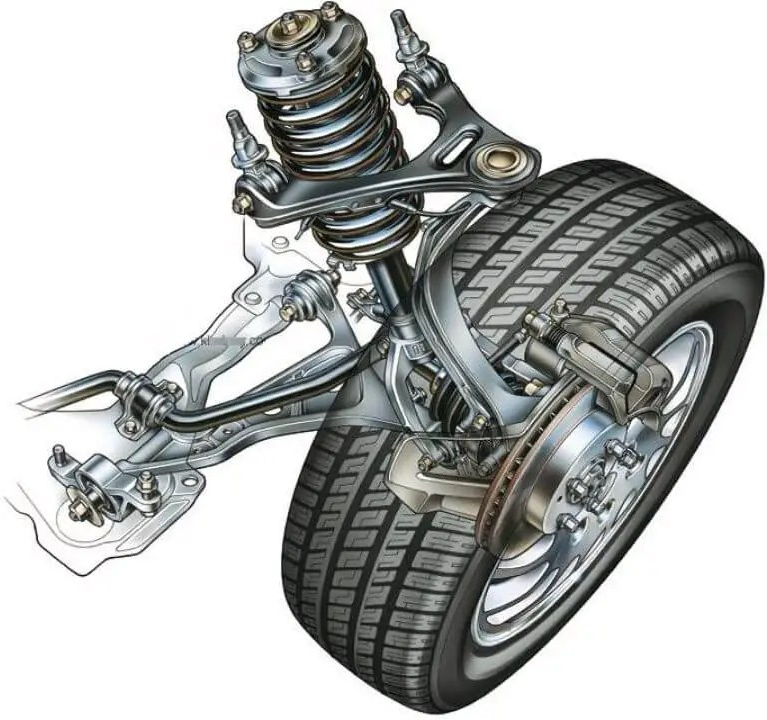
\includegraphics[width=1.0\textwidth]{car_suspension.png}
  \end{minipage}
\end{frame}

\begin{frame}{K\&C analysis}{Introduction}
  \begin{minipage}[c]{0.55\linewidth}
    The \textbf{kinematics} and \textbf{compliance} of the suspension system are \dots
    \begin{enumerate}
      \item the \textbf{motion} and \textbf{deformation} of the system
      \item key aspects of the \textbf{design} of the system \vspace*{1.0em}
    \end{enumerate}
    \begin{center}\begin{minipage}{6.0cm}\begin{block}{}
      \centering
      \hi{Kinematics and compliance are what is needed to describe the suspension in a vehicle model}
    \end{block}\end{minipage}\end{center}
  \end{minipage}
  \hfill
  \begin{minipage}[c]{0.4\linewidth}
    \centering
    \vspace{-2.0em}
    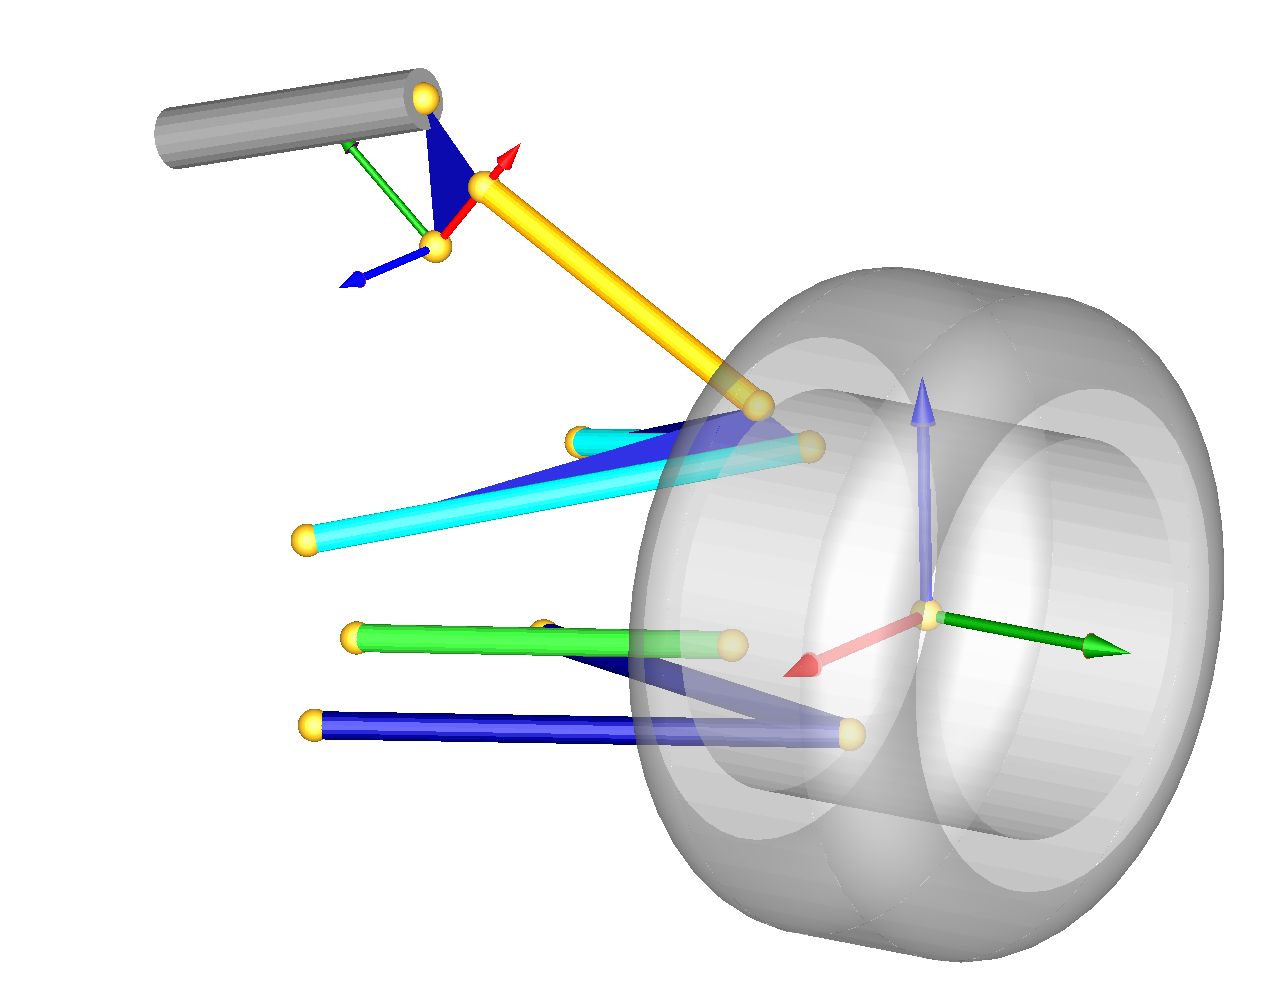
\includegraphics[width=1.0\linewidth]{kinematic_model.png} \\[-4em]
    \hspace*{-10em}
    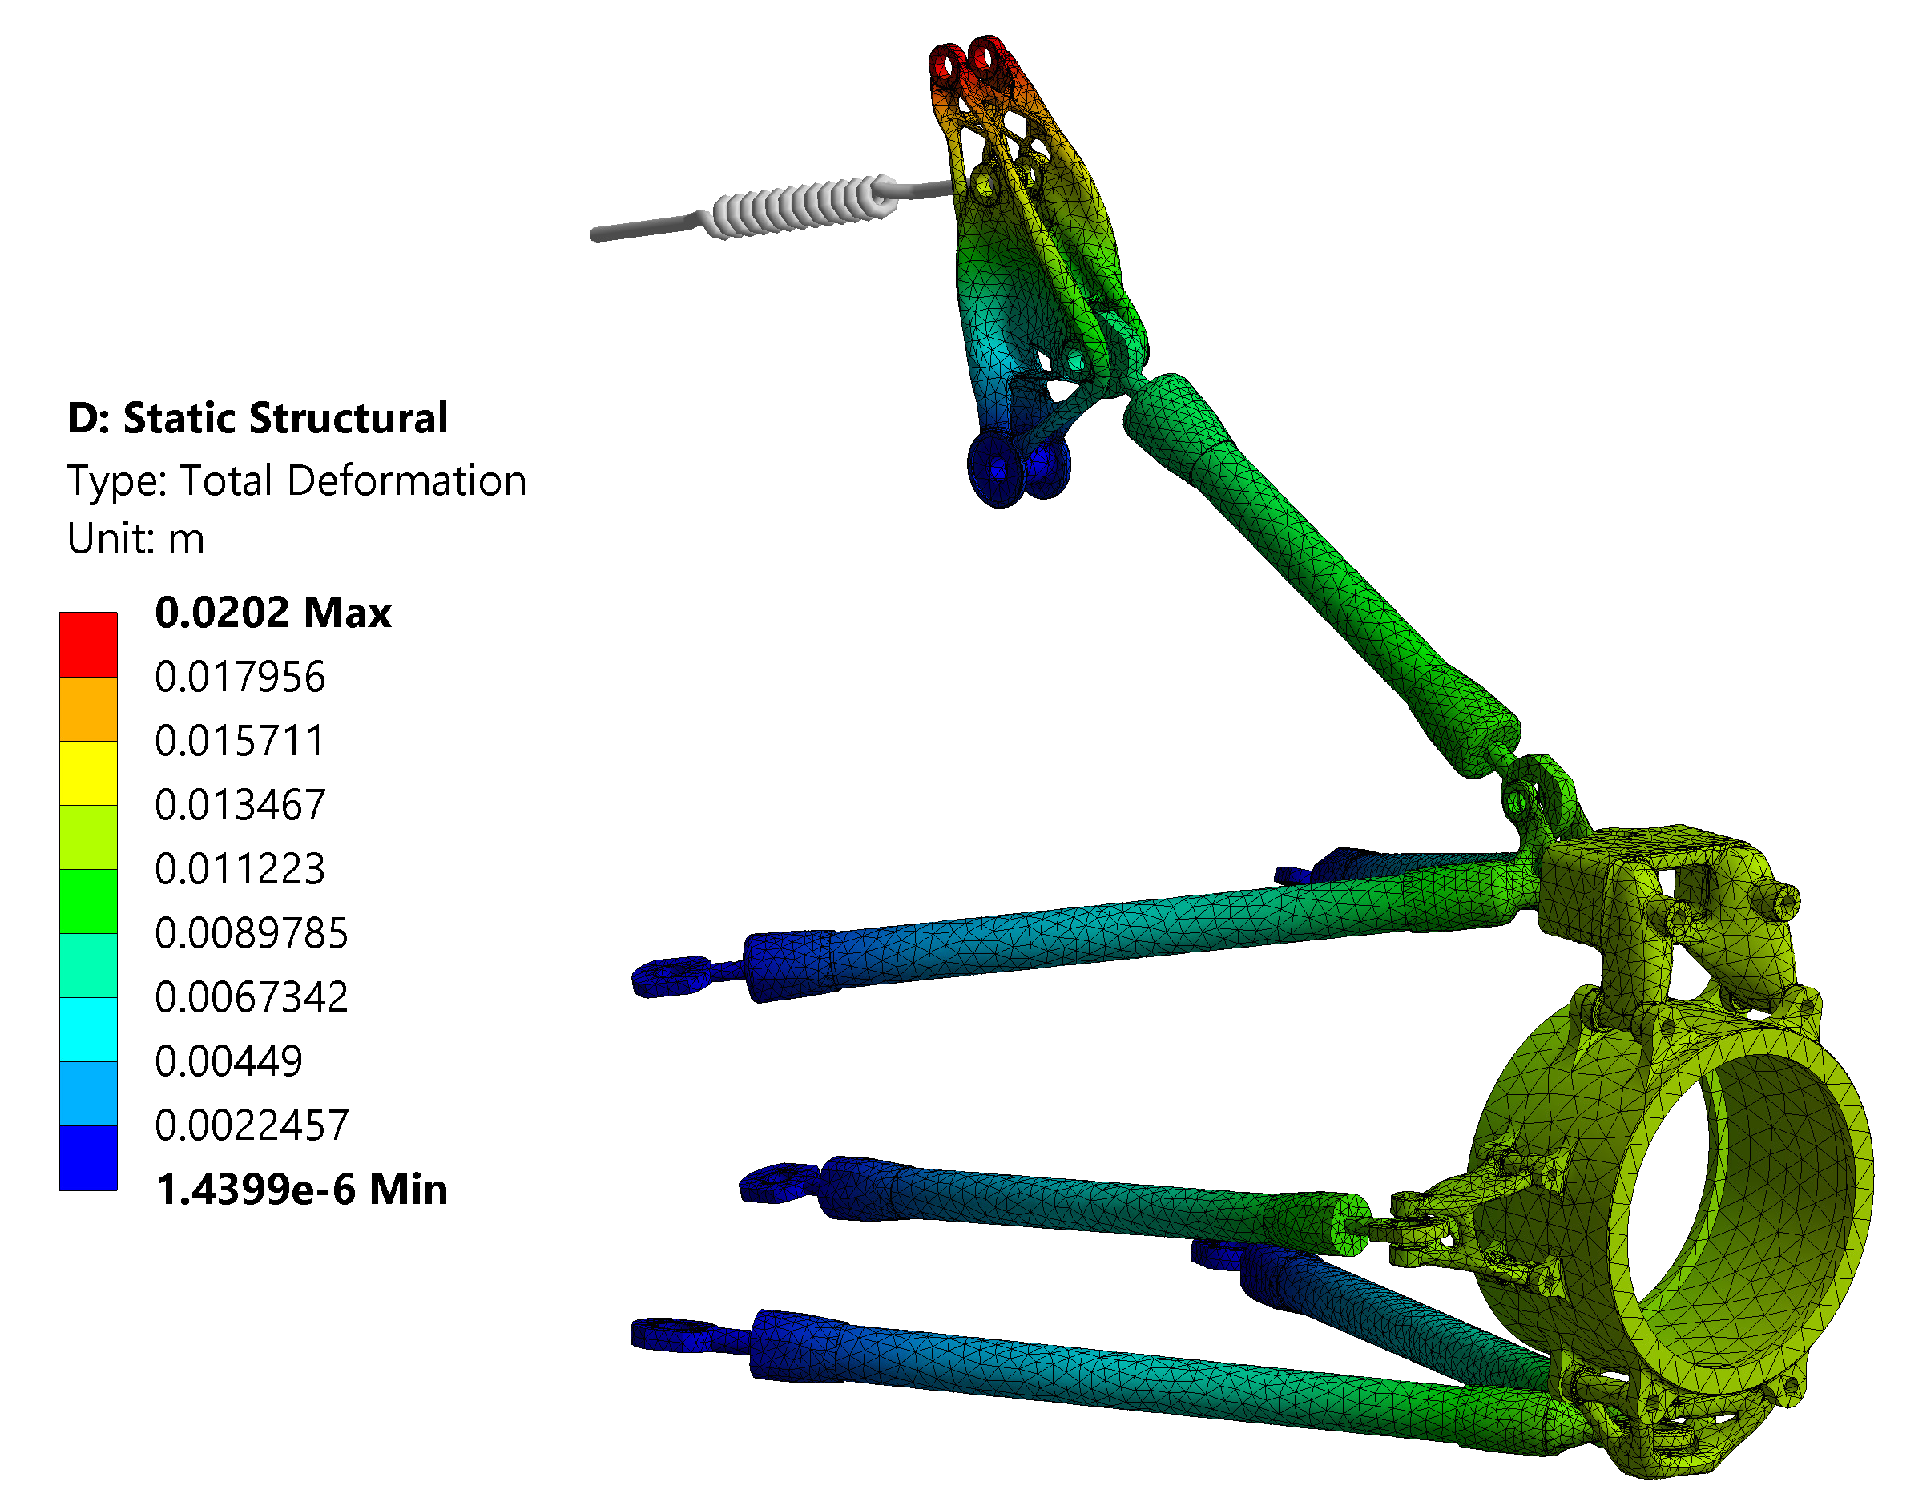
\includegraphics[width=0.7\linewidth, trim={9cm 0cm 0cm 0cm}, clip]{compliance_model.pdf}
  \end{minipage}
\end{frame}

\begin{frame}{K\&C analysis}{State-of-the-art solutions}
  \begin{center}
    \begin{tabular}{lcccc}
      \toprule
      \textbf{Methods} & \textbf{Real-Time} & \textbf{Accuracy} & \textbf{Parametric} & \textbf{Easy to Setup} \\
      \midrule
      FE methods & \mycrossmark & \mycheckmark & \mycrossmark  & \mycrossmark \\
      Map-based methods & \mycheckmark & \mydotmark & \mycrossmark & \mycheckmark \\
      Flexible multibody & \mydotmark & \mycheckmark & \mydotmark & \mycrossmark \\
      What we aim to \dots & \mycheckmark & \mydotmark & \mycheckmark & \mycheckmark \\
      \bottomrule
    \end{tabular}
  \end{center}
  \vspace{0.5cm}
  \begin{center}
    \emph{Legend}: \mycheckmark{} satisfied, \mydotmark{} satisfied with limitations, and \mycrossmark{} not satisfied.
  \end{center}
\end{frame}

\begin{frame}{Symbolic computation}{Finite element method problem}
  \begin{itemize}
    \item Symbolic computation can be applied to the \textbf{finite element (FE) method}. \\
    \item \textbf{Stiffness matrix}, \textbf{load vector}, and \textbf{boundary conditions} are defined symbolically. \\
    \begin{equation*}
      \begin{bmatrix}
        \mathbf{K}_{ff} & \mathbf{K}_{fs} \\
        \mathbf{K}_{sf} & \mathbf{K}_{ss}
      \end{bmatrix} \begin{bmatrix}{c}
        \mathbf{d}_{f} \\
        \mathbf{d}_{s}
      \end{bmatrix} = \begin{bmatrix}{c}
        \mathbf{f}_{f} \\
        \mathbf{f}_{s}
      \end{bmatrix}
      \quad \xrightarrow[\text{method}]{\text{direct stiffness}} \quad
      \begin{array}{c}
        \mathbf{d}_{f} = \mathbf{K}_{ff}^{-1}\,\left(\mathbf{f}_{f} - \mathbf{K}_{fs}\,\mathbf{d}_{s}\right) \\
        \mathbf{f}_{s} = \mathbf{K}_{sf}\,\mathbf{d}_{f} + \mathbf{K}_{ss}\,\mathbf{d}_{s}
      \end{array}
    \end{equation*}
    \begin{enumerate}
      \item Possibility to \textbf{evaluate} the system \textbf{without} the need to ``\textbf{reassemble}'' the system \\
      \item Parametric formulation \\
      \item Symbolic solution of the structure deformations and reaction forces \\
    \end{enumerate}
  \end{itemize}
  \begin{center}\begin{minipage}{10.75cm}\begin{block}{}
    \centering
    FE method $\quad \xrightarrow[\text{computation}]{\text{symbolic}} \quad$ Symbolic FE model + \textcolor{mycolor5}{\textbf{A lot of flexibility!}}
  \end{block}\end{minipage}\end{center}
  \begin{itemize}
    \item We combined all these features in the \Maple{} \TrussMe{} library (open-source)
  \end{itemize}
\end{frame}

\begin{frame}{Symbolic computation}{Linear algebra}
  \begin{itemize}
    \item Symbolic matrix factorization is used for the computation of the linear system \textbf{solutions}
    \begin{equation*}
      \mathbf{d}_{f} = \mathbf{K}_{ff}^{-1}\,\left(\mathbf{f}_{f} - \mathbf{K}_{fs}\,\mathbf{d}_{s}\right)
    \end{equation*}
    \begin{bbox}[Problem]
      \Maple matrix factorizations have \textbf{limited capabilities}.
    \end{bbox}
    \item We developed the \texttt{LAST} symbolic matrix factorization toolbox capable of \dots  \\
    \begin{enumerate}
      \item extending \Maple factorization capabilities \\
      \item introducing \textbf{veiling variables} not to increase the expressions size (through \texttt{LEM} toolbox) \\
      \item performing efficient LU, Fraction-Free LU, QR, and Gauss-Jordan factorizations with limited \textbf{expresion swell} \\
    \end{enumerate}
  \end{itemize}
\end{frame}

\begin{frame}{Symbolic computation}{Mixed symbolic/numerical solution}
  \begin{itemize}
    \item \textbf{Symbolic} solution is not always possible due to
    \begin{enumerate}
      \item capability of the symbolic kernel to handle \textbf{complicated} expressions
      \item \textbf{non-linear} or mathematically \textbf{unsolvable} problems
    \end{enumerate}
     \item Symbolic computation should be exploited as much as possible!
  \end{itemize}
  \begin{center}\begin{minipage}{1.0\textwidth}\begin{block}{}
    \centering
    FE model $\quad \xrightarrow[\text{computation}]{\text{symbolic}} \quad$ \hspace*{1.05cm}\textcolor{mycolor2}{\textbf{Stop}}\hspace*{1.05cm} $\quad \xrightarrow[\text{generation}]{\text{code}} \quad$ \begin{minipage}[c]{0.27\linewidth}\begin{center}{\textbf{Efficient} numeric \\ FE model solution}\end{center}\end{minipage}
  \end{block}\end{minipage}\end{center}
  \begin{center}\begin{minipage}{1.0\textwidth}\begin{block}{}
    \centering
    FE model $\quad \xrightarrow[\text{computation}]{\text{symbolic}} \quad$ \textcolor{mycolor5}{\textbf{Symbolic solution}} $\quad \xrightarrow[\text{generation}] {\text{code}} \quad$ \begin{minipage}[c]{0.27\linewidth}\begin{center}{\textbf{Fastest} \\ numeric evaluation!}\end{center}\end{minipage}
  \end{block}\end{minipage}\end{center}
  \begin{itemize}
    \item K\&C{} of suspensions are computed through a \textbf{mixed} symbolic/numerical approach
  \end{itemize}
\end{frame}

\begin{frame}{Suspensions symbolic modeling}{Case study}
  The modeled suspension is a \textbf{double wishbone} suspension system of the \textbf{Formula SAE} vehicle of \emph{E-Agle Trento Racing Team} (University of Trento) \\[1.0em]
  \begin{center}
    \begin{minipage}[c]{0.65\textwidth}
      \centering
      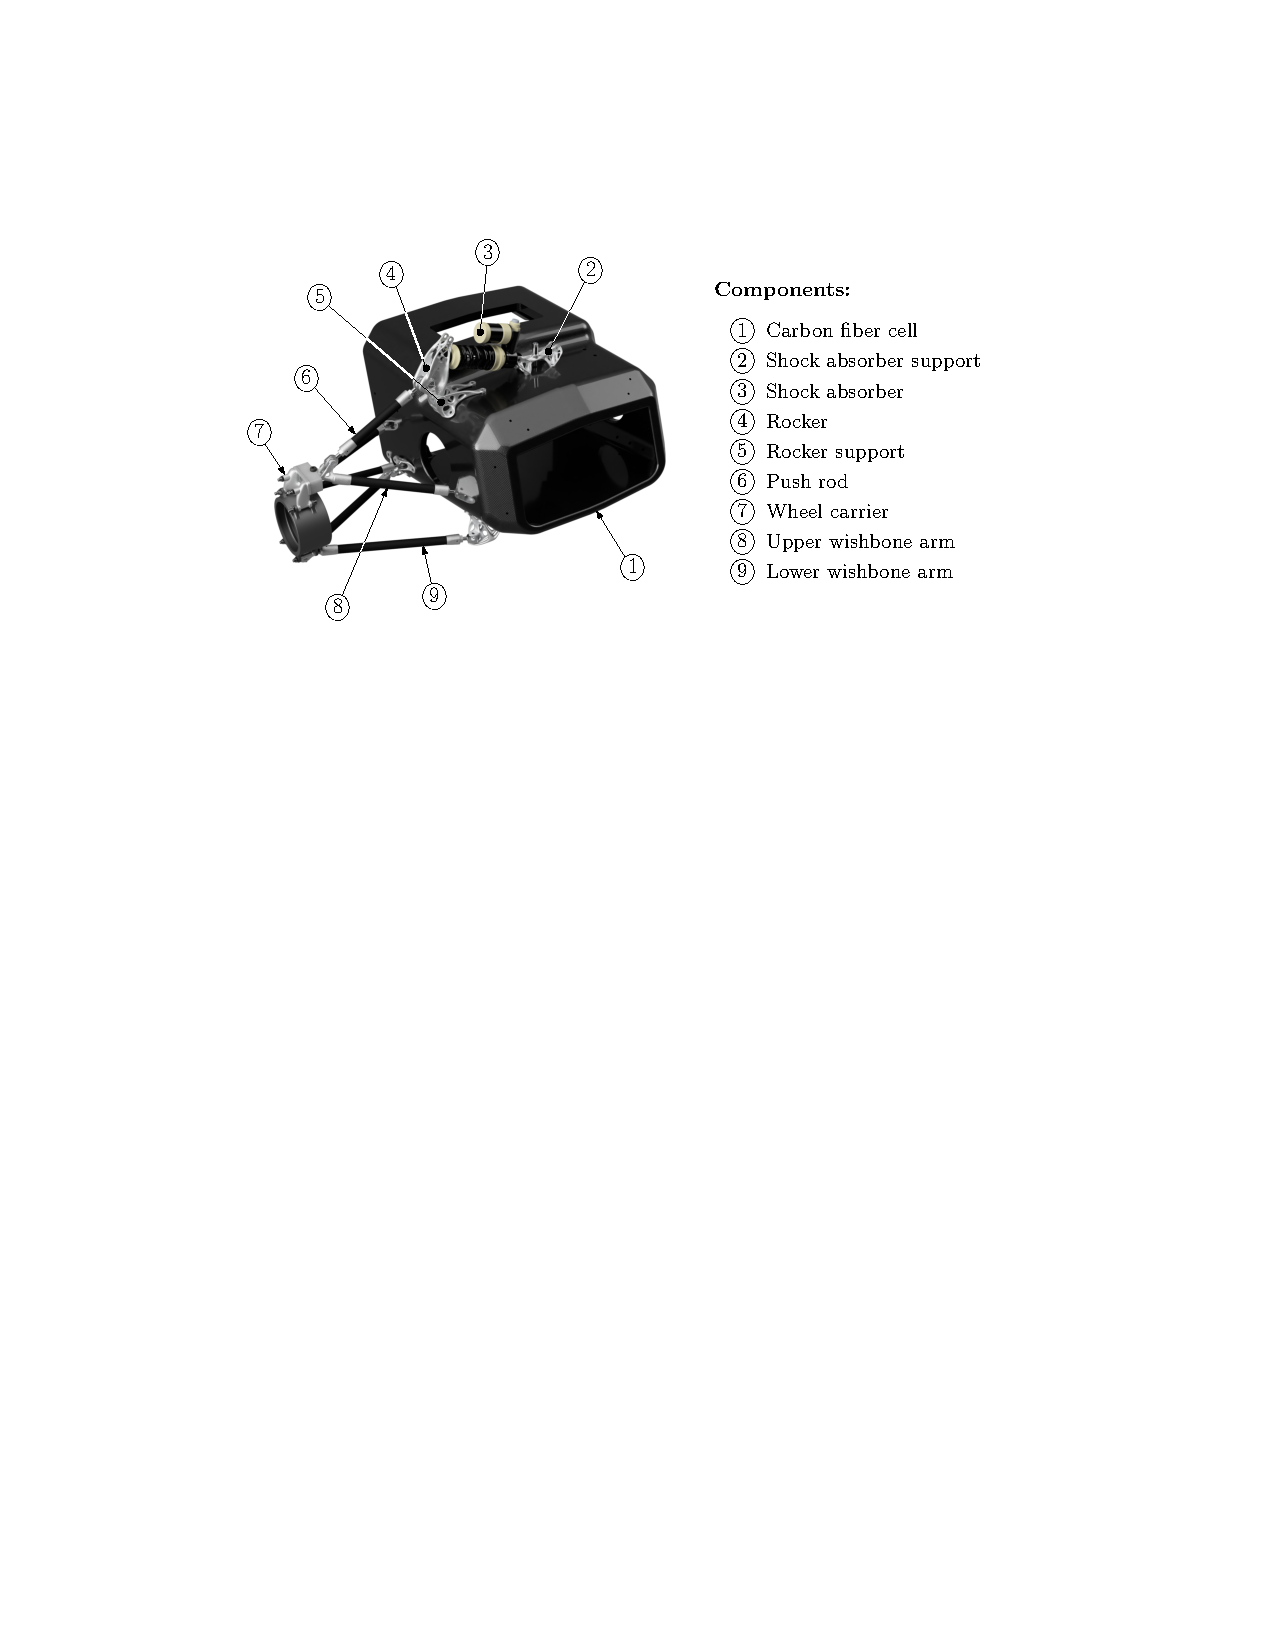
\includegraphics[width=1.0\textwidth]{render_all.pdf}
    \end{minipage}
    \hspace*{1em}
    \begin{minipage}[c]{0.25\textwidth}
      \centering
      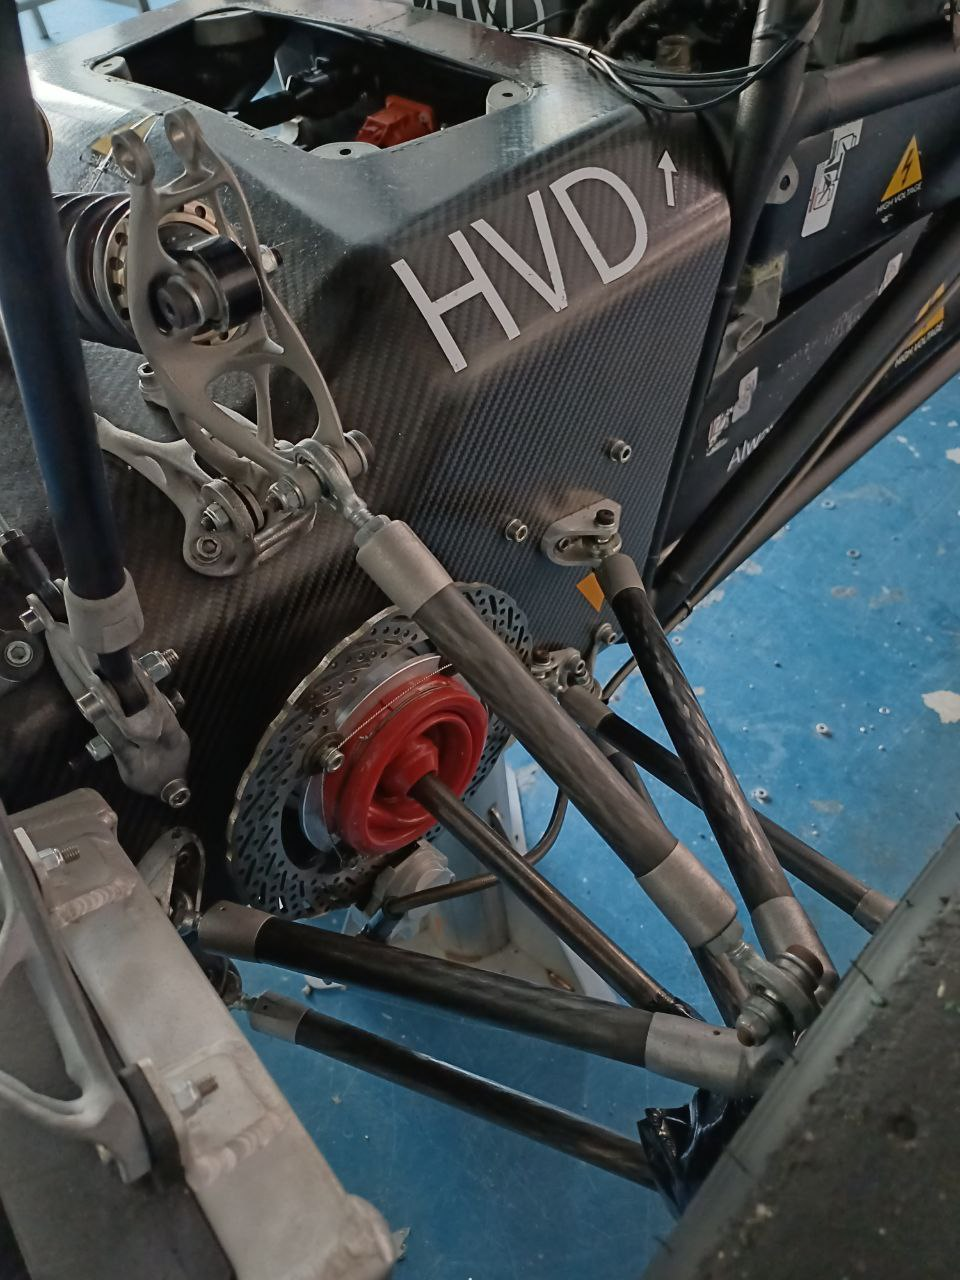
\includegraphics[width=1.0\textwidth]{fsae.jpeg}
    \end{minipage}
  \end{center}
\end{frame}

\begin{frame}{Suspensions symbolic modeling}{Rigid multibody \& FE models}
  \begin{minipage}[c]{0.55\linewidth}
    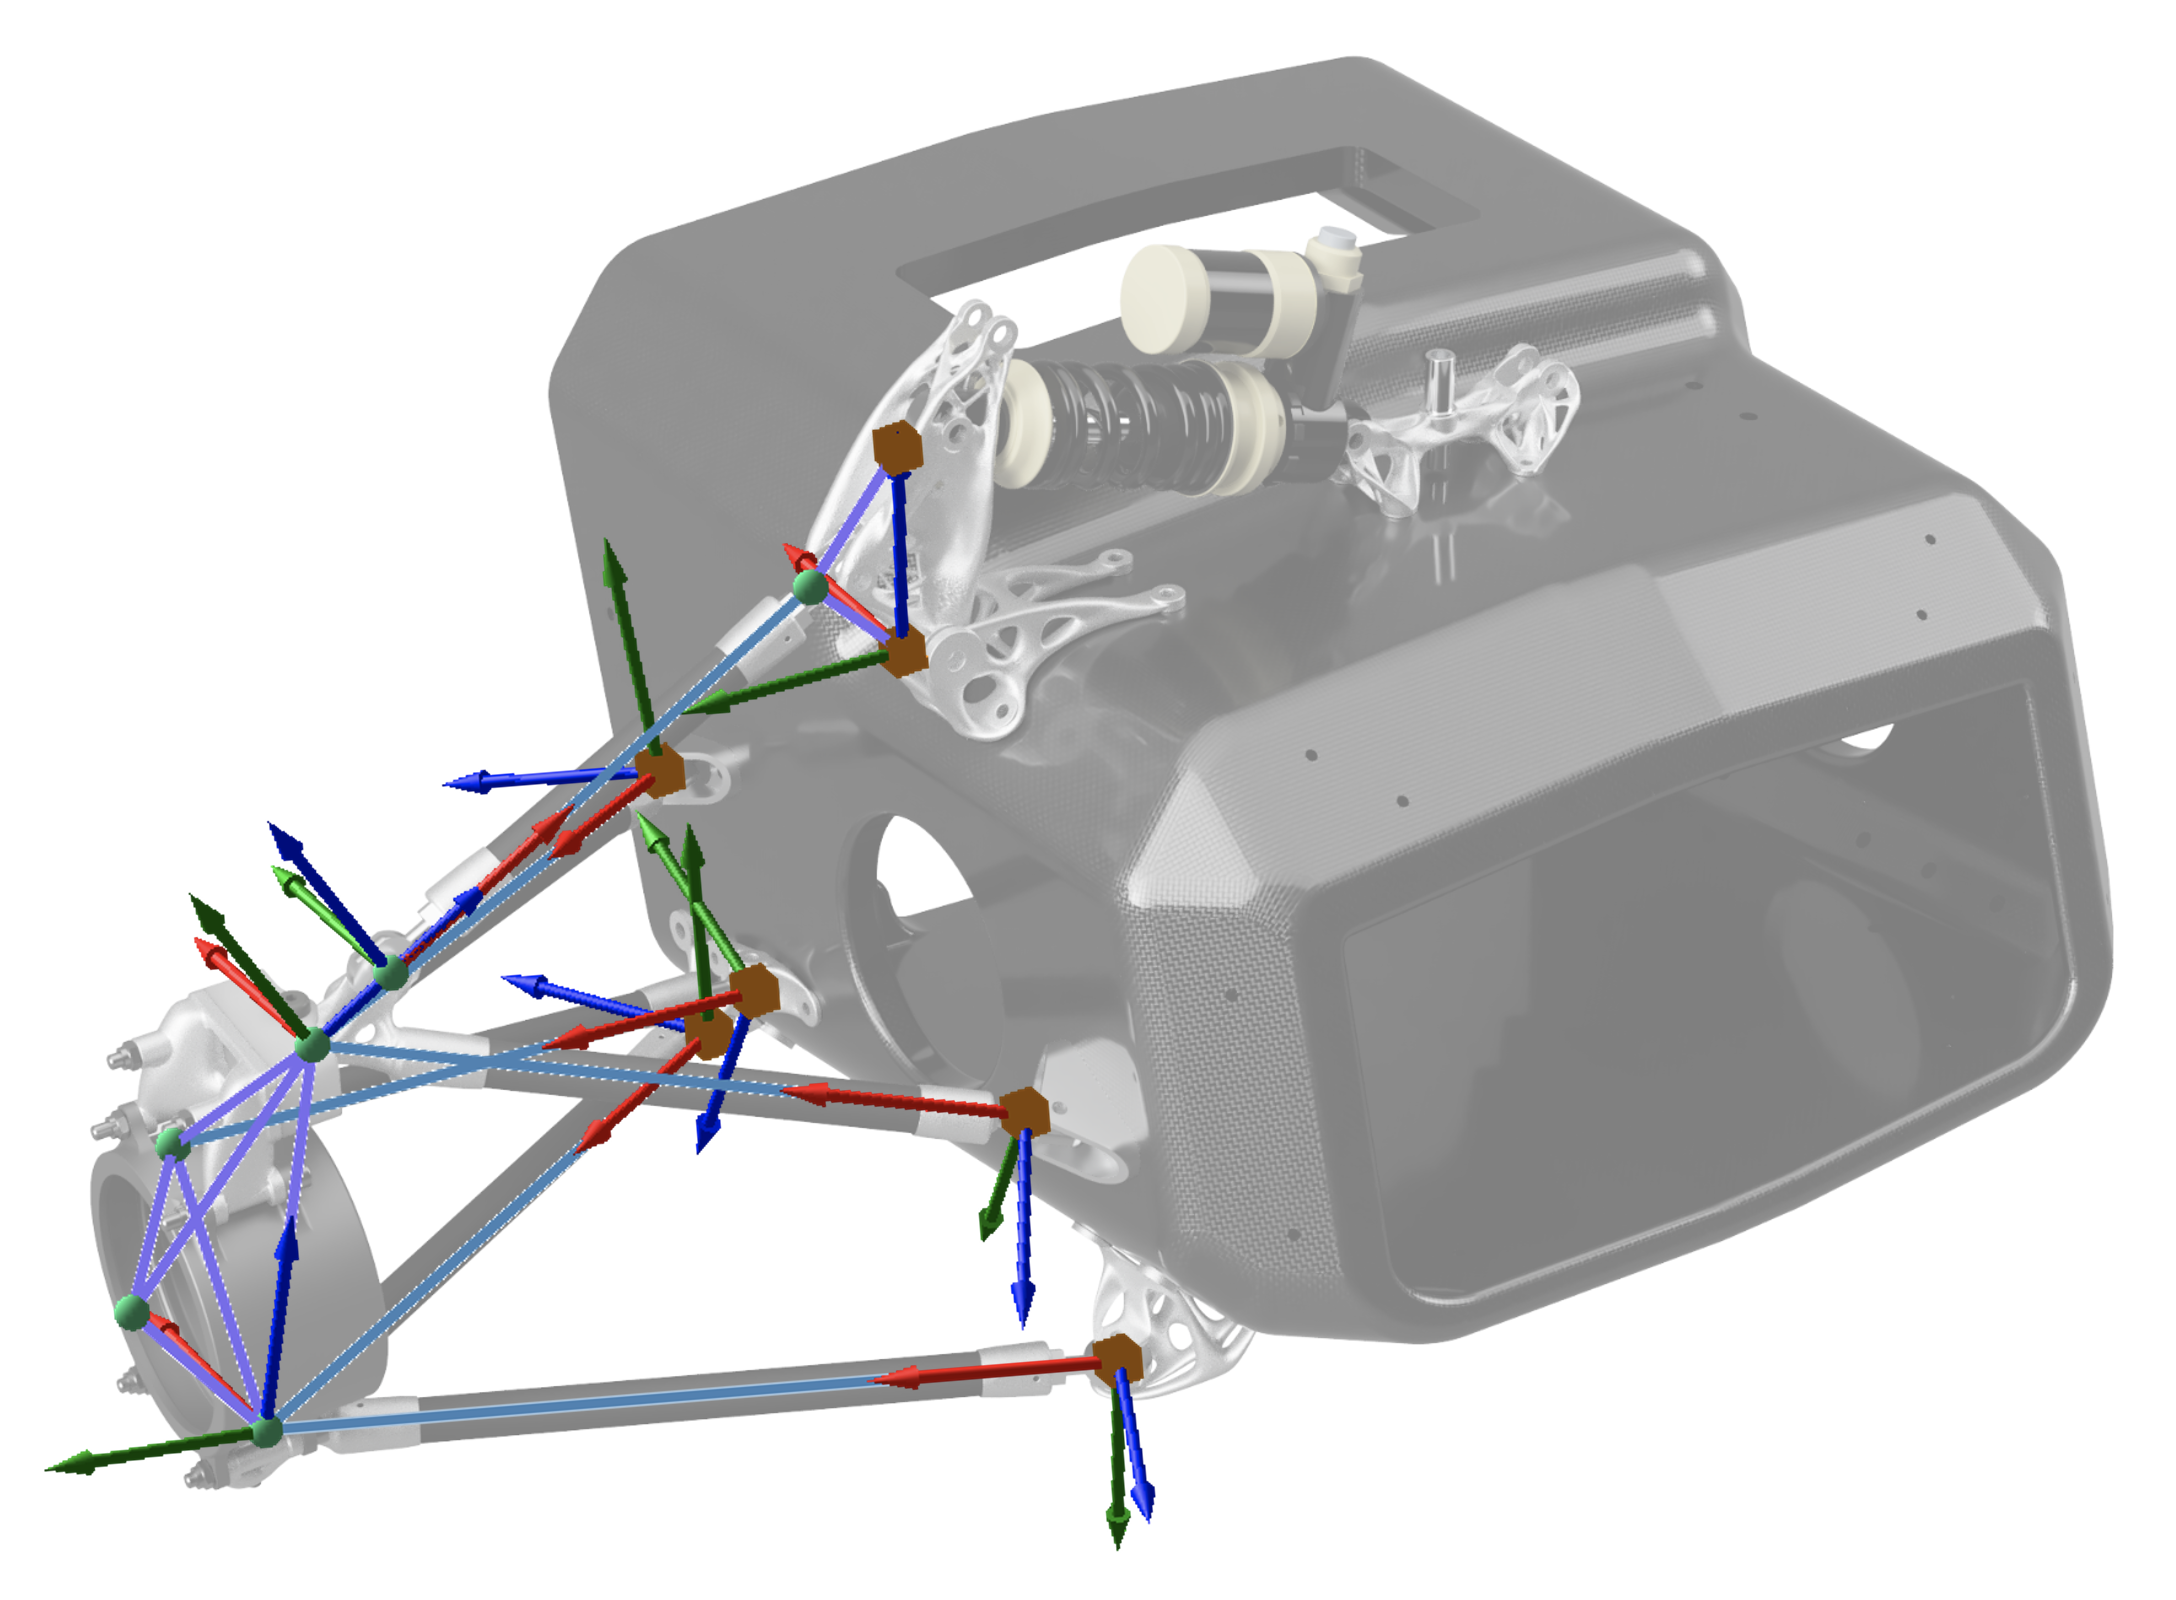
\includegraphics[width=0.8\textwidth]{fade_overview.png}\\
    \hi{138 DoFs symbolic FE model}
  \end{minipage}
  \begin{minipage}[c]{0.40\linewidth}
    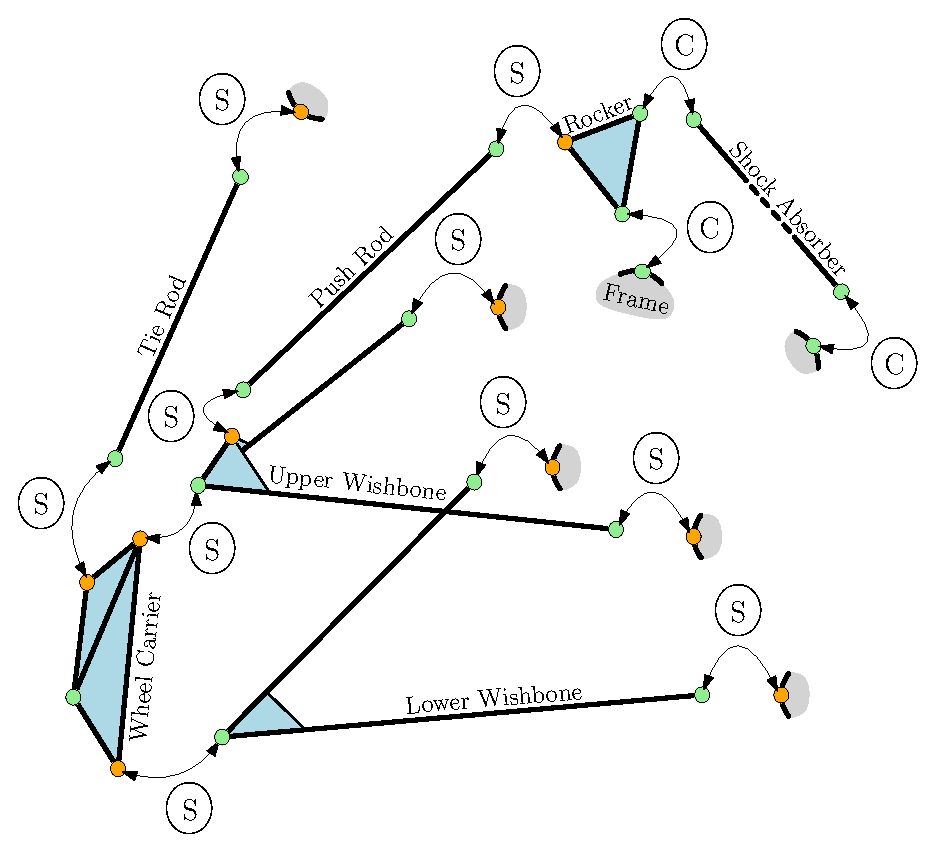
\includegraphics[width=1.0\textwidth]{constraints.eps}
  \end{minipage}
\end{frame}

\begin{frame}{Simulation results}{Static analysis}
  \vspace{-1.75em}
  \begin{center}
    \begin{minipage}[c]{0.485\linewidth}
      \centering{\textbf{Static translations}} \\[0.2em]
      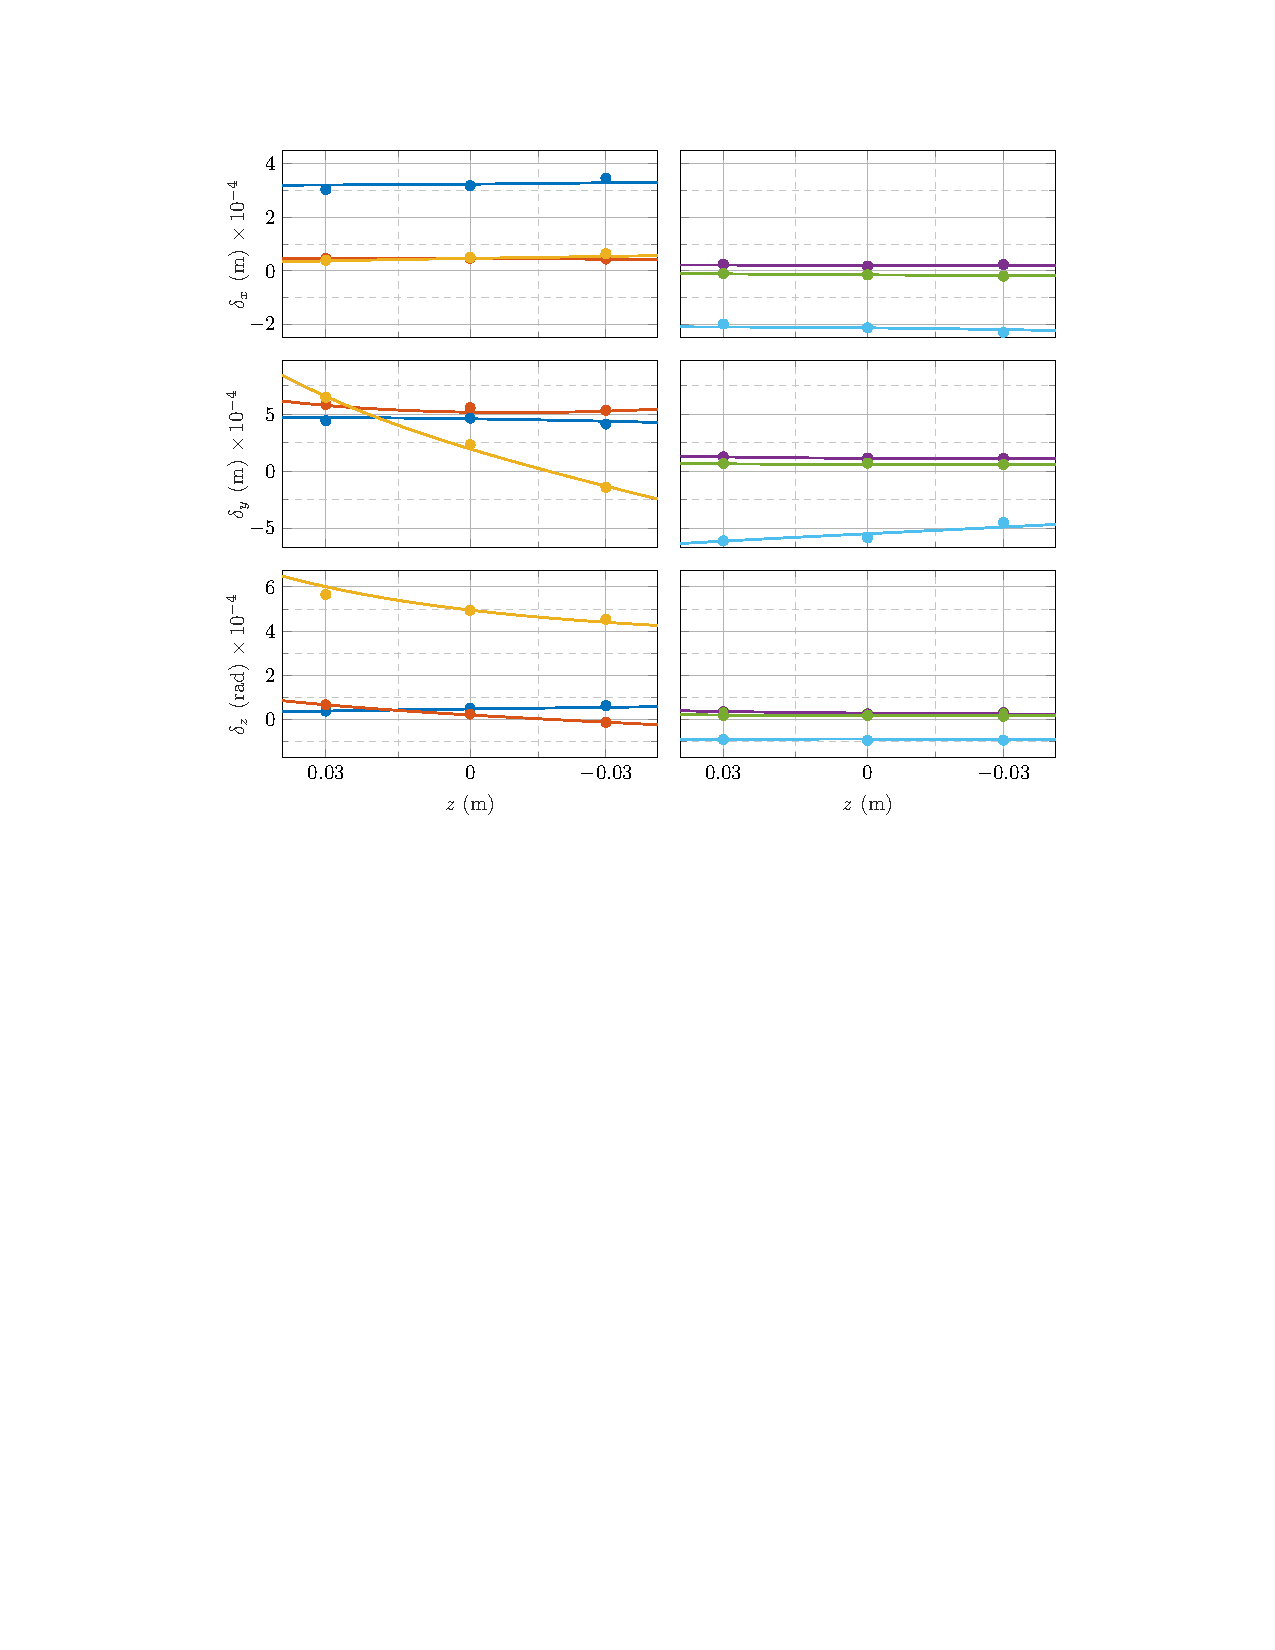
\includegraphics[width=1.0\textwidth]{static_translations.pdf}
    \end{minipage}
    \begin{minipage}[c]{0.485\linewidth}
      \centering{\textbf{Static rotations}} \\[0.2em]
      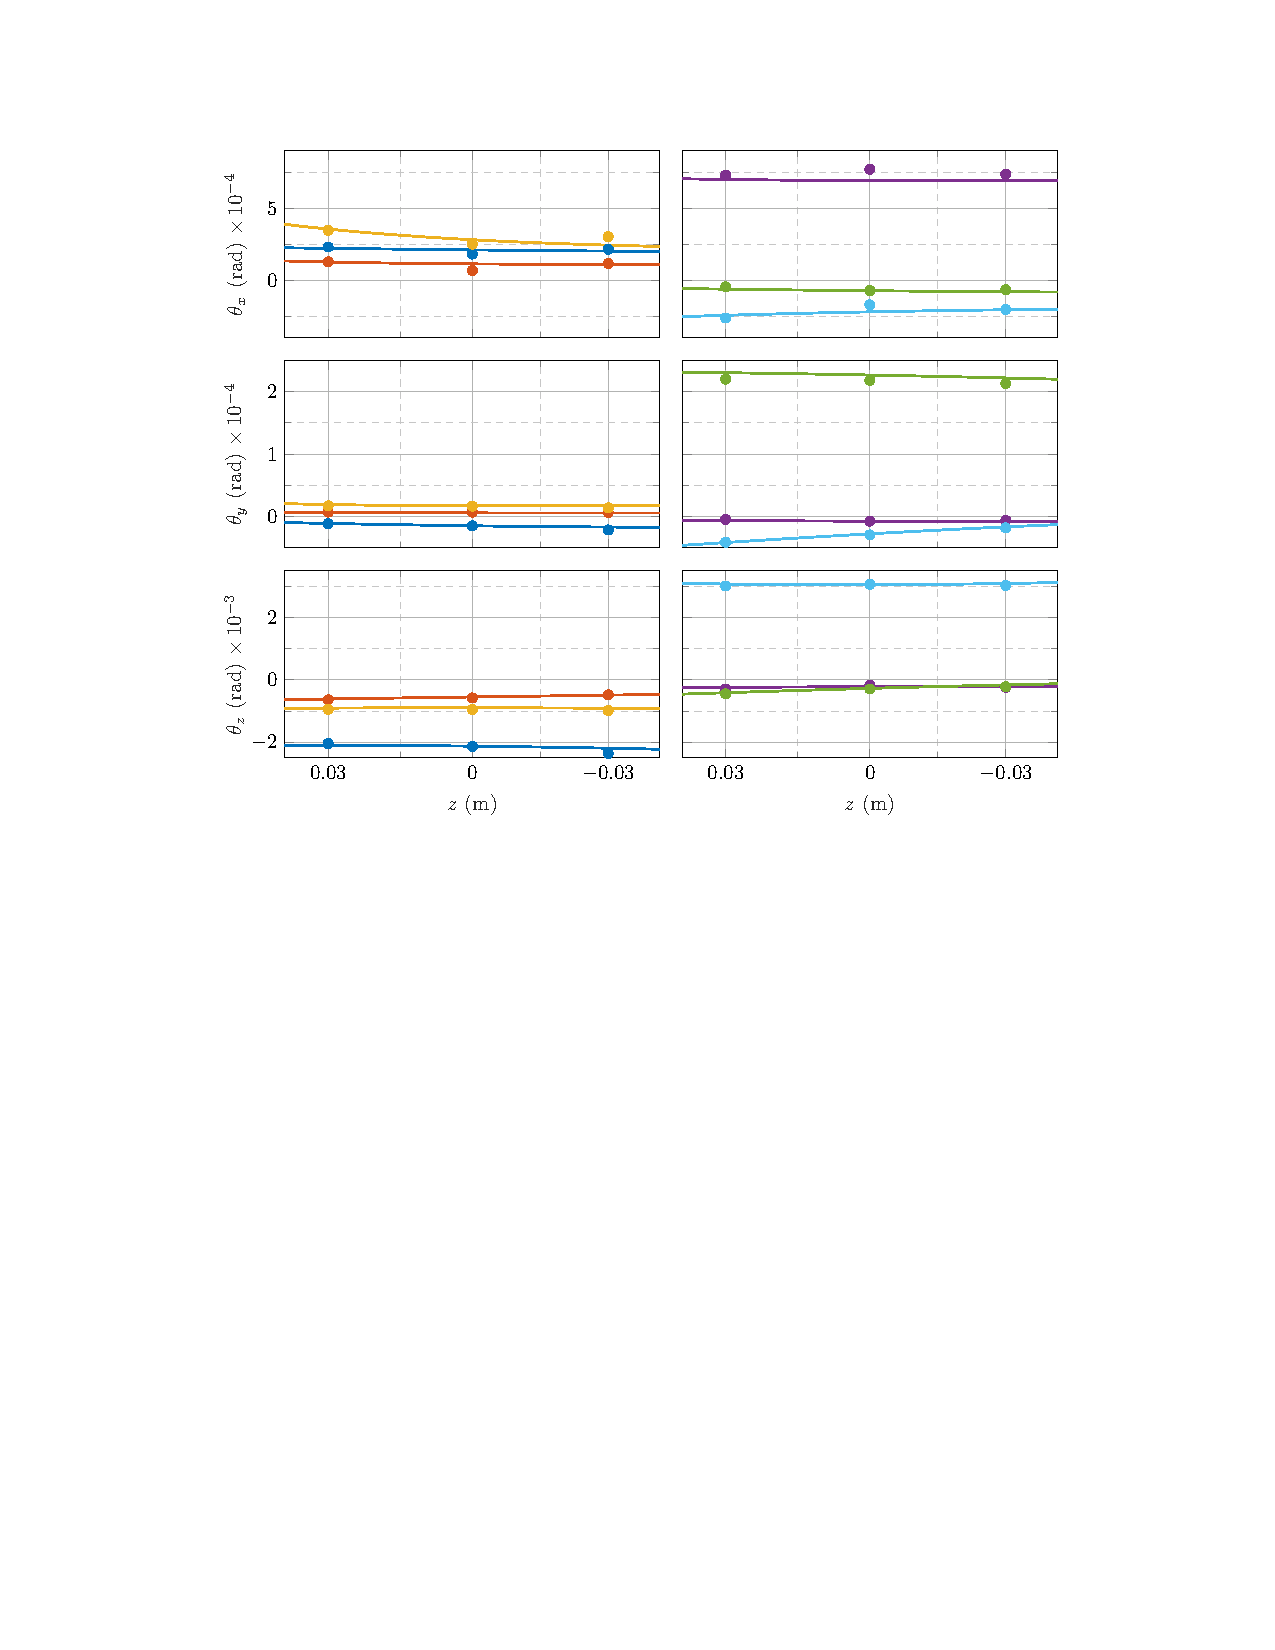
\includegraphics[width=1.0\textwidth]{static_rotations.pdf}
    \end{minipage}
    \raggedright{\footnotesize{\emph{Legend:} \TrussMe{} solution (\emph{solid lines}), \Ansys{} data (\emph{bullets}). \\ {\color{mycolor1}$\blacksquare$} $F_x =$ \SI{4000}{\newton}, {\color{mycolor2}$\blacksquare$} $F_y =$ \SI{4000}{\newton}, {\color{mycolor3}$\blacksquare$} $F_z =$ \SI{4000}{\newton}, with $M_x = M_y = M_z =$ \SI{0}{\newton\meter}. \\ {\color{mycolor4}$\blacksquare$} $M_x =$ \SI{400}{\newton\meter}, {\color{mycolor5}$\blacksquare$} $M_y =$ \SI{400}{\newton\meter}, {\color{mycolor6}$\blacksquare$} $M_z =$ \SI{400}{\newton\meter}, with $F_x = F_y = F_z =$ \SI{0}{\newton}}}
  \end{center}
\end{frame}

\begin{frame}{Suspensions symbolic modeling}{Modeling assumptions}
  \begin{minipage}[t]{0.32\linewidth}
    \centering
    \hi{No compliance}\\[3.4em]
    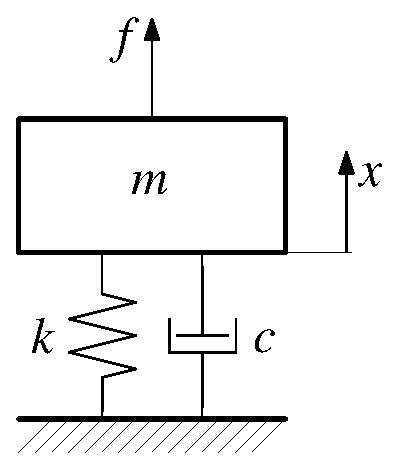
\includegraphics[width=0.5\textwidth]{system_no_compliance.eps}
    \begin{equation*}
      m \ddot{x} + c \dot{x} + k x = f
    \end{equation*}
  \end{minipage}
  \hfill
  \begin{minipage}[t]{0.32\linewidth}
    \centering
    \hi{Quasi-static compliance}\\[0.5em]
    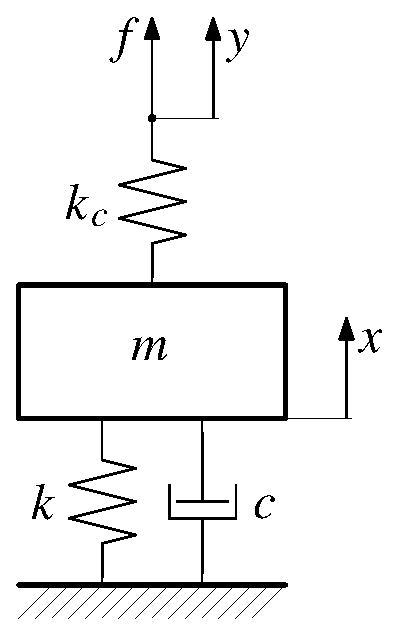
\includegraphics[width=0.5\textwidth]{system_superposition.eps}
    \begin{equation*}
      \begin{cases}
        y = x + d  \\
        k_c d = f  \\
        m \ddot{x} + c \dot{x} + k x = f
      \end{cases}
    \end{equation*}
  \end{minipage}
  \hfill
  \begin{minipage}[t]{0.32\linewidth}
    \centering
    \hi{Dynamic compliance}\\[0.52em]
    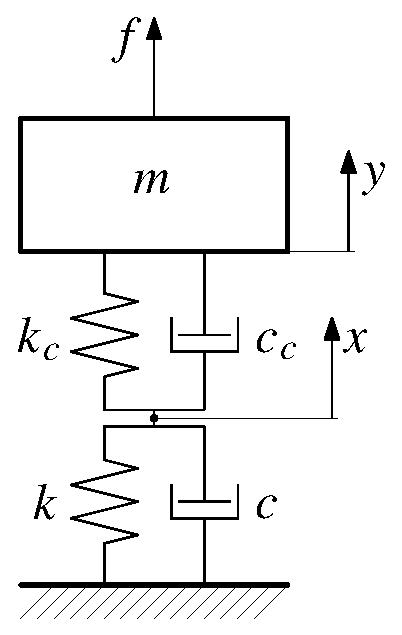
\includegraphics[width=0.5\textwidth]{system_real.eps}
    \begin{equation*}
      \begin{cases}
        y = x + d \\
        k x + c \dot{x} = k_c d + c_c \dot{d} \\
        m \ddot{y} = k_c d + c_c \dot{d} + f
      \end{cases}
    \end{equation*}
  \end{minipage}
\end{frame}

\begin{frame}{Suspensions symbolic modeling}{Frequency response}
  \centering{The \textbf{frequency response} of the system is influenced by the \textbf{decoupling} strategy.} \\[0.5em]
  \begin{columns}
    \begin{column}[c]{0.7\textwidth}
      \begin{itemize}
        \item[{\color{mycolor1}$\blacksquare$}] no compliance
          \vspace{-0.2cm}%
          {\scriptsize{
          \begin{flalign*}
          \dfrac{\ddot{Y}(s)}{F(s)} = \dfrac{s^2}{ms^2 + cs + k}&&
          \end{flalign*}
          }}
        \item[{\color{mycolor2}$\blacksquare$}] quasi-static compliance
        \vspace{-0.2cm}%
          {\scriptsize{
          \begin{flalign*}
          \dfrac{\ddot{Y}(s)}{F(s)} = \dfrac{s^2}{ms^2 + cs + k} + \dfrac{s^2}{k_c} \quad \substack{\omega_{n} = \sqrt{\dfrac{k}{m}} \\[1em] \omega_z = \sqrt{\dfrac{k + k_c}{m}}}&&
          \end{flalign*}
          }}
        \item[{\color{mycolor3}$\blacksquare$}] dynamic compliance
          \vspace{-0.2cm}%
          {\scriptsize{
          \begin{flalign*}
          \dfrac{\ddot{Y}(s)}{F(s)} = \dfrac{(c \!+\! c_c)s^3 + (k \!+\! k_c)s^2}{m(c \!+\! c_c)s^3 + (c\,c_c + m(k \!+\! k_c))s^2 + (k_c\,c \!+\! k\,c_c)s + k\,k_c}&&
          \end{flalign*}
          }}
      \end{itemize}
    \end{column}%
    \hspace{-4.5cm}%
    \begin{column}[c]{0.4\textwidth}
      \vspace{-1.0cm}
      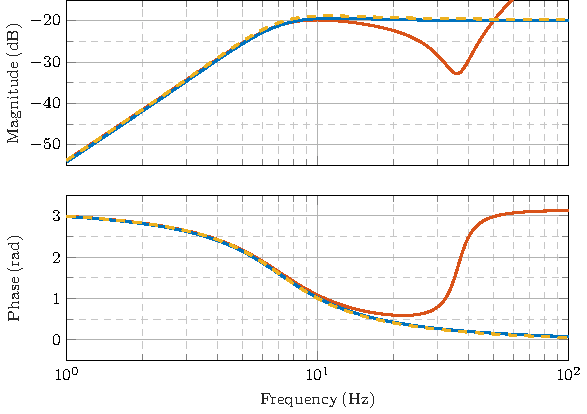
\includegraphics[width=1.05\linewidth]{tf_theory.pdf}
    \end{column}
  \end{columns}
\end{frame}

\begin{frame}{Simulation results}{Frequency response}
  \begin{minipage}[c]{0.69\linewidth}
    \centering{\textbf{Acceleration/force frequency response}} \\[0.25em]
    {\footnotesize{
    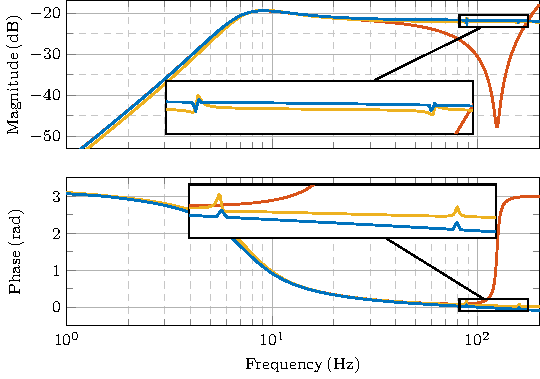
\includegraphics[width=0.8\textwidth]{frequency_tz.pdf}
    \begin{center}
      \emph{Legend:}
      {\color{mycolor1}$\blacksquare$} MB with compliance dynamic, {\color{mycolor2}$\blacksquare$} MB and steady-state compliance, {\color{mycolor3}$\blacksquare$} \Ansys \ac{FE} modal analysis.
    \end{center}
    }}
  \end{minipage}
  \hfill
  \begin{minipage}[c]{0.3\linewidth}
    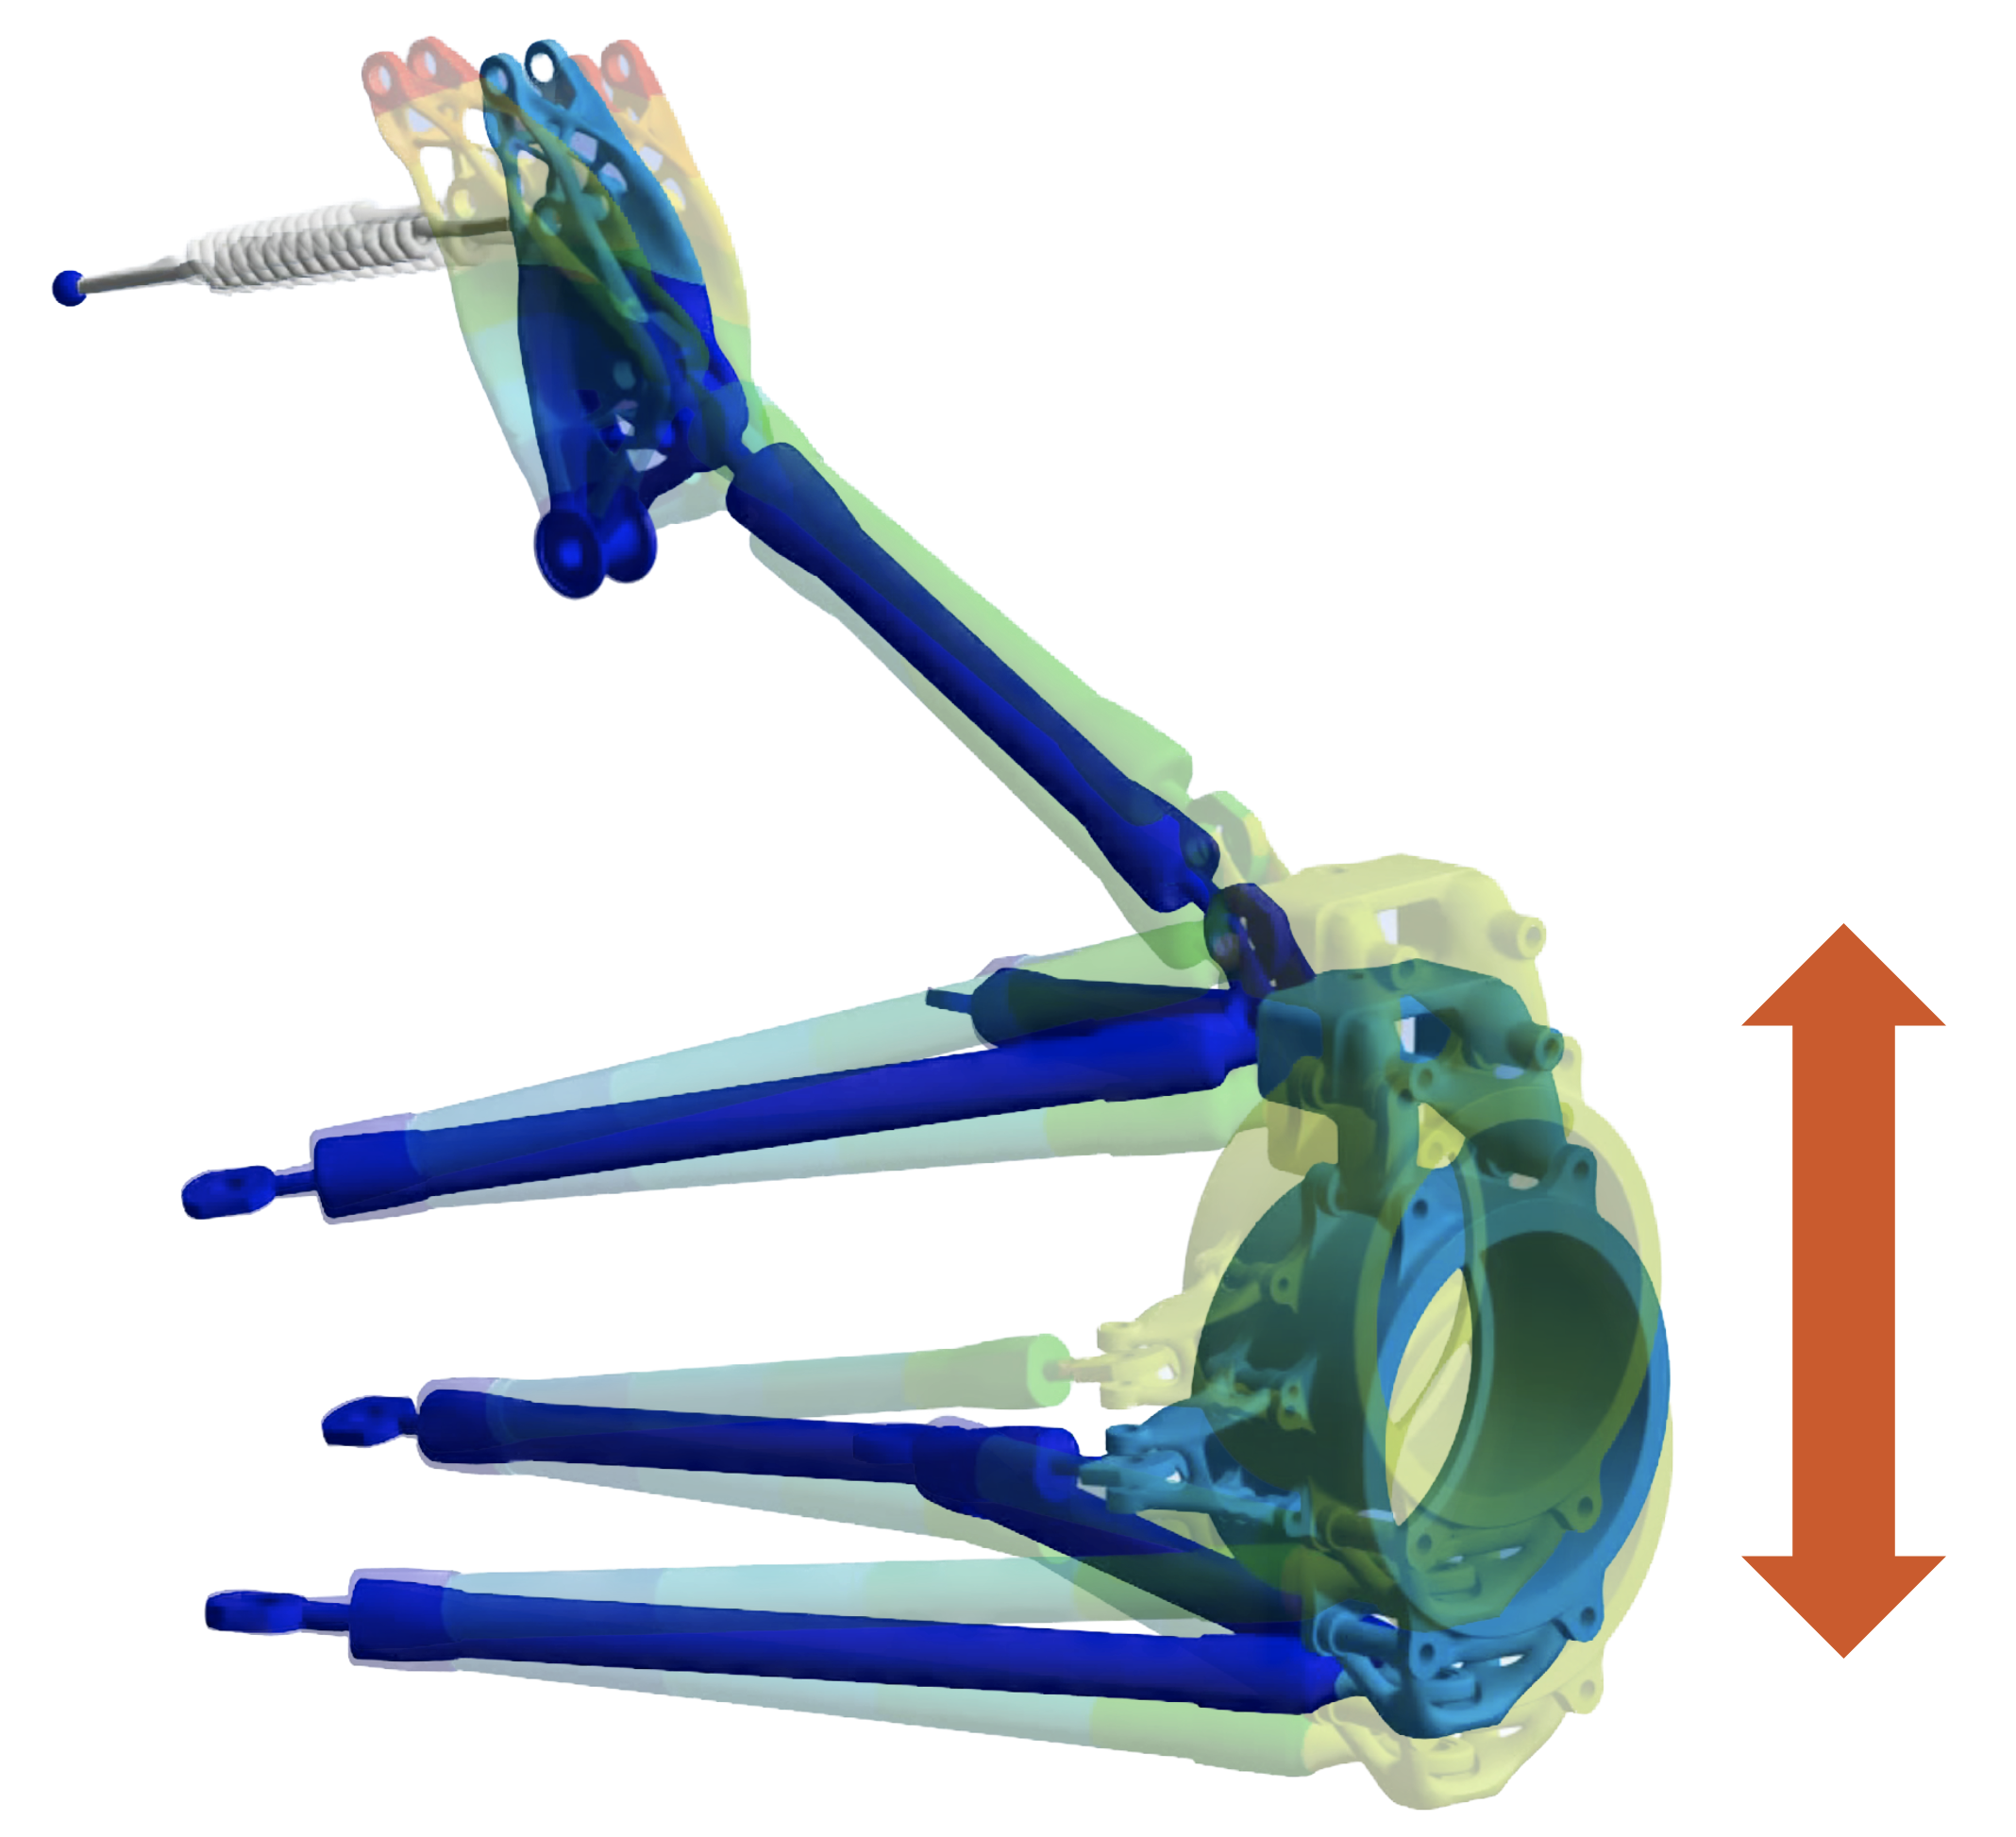
\includegraphics[width=0.5\linewidth]{mode1.png} \raisebox{2.0em}{\small{$f = 7.6$ Hz}} \\
    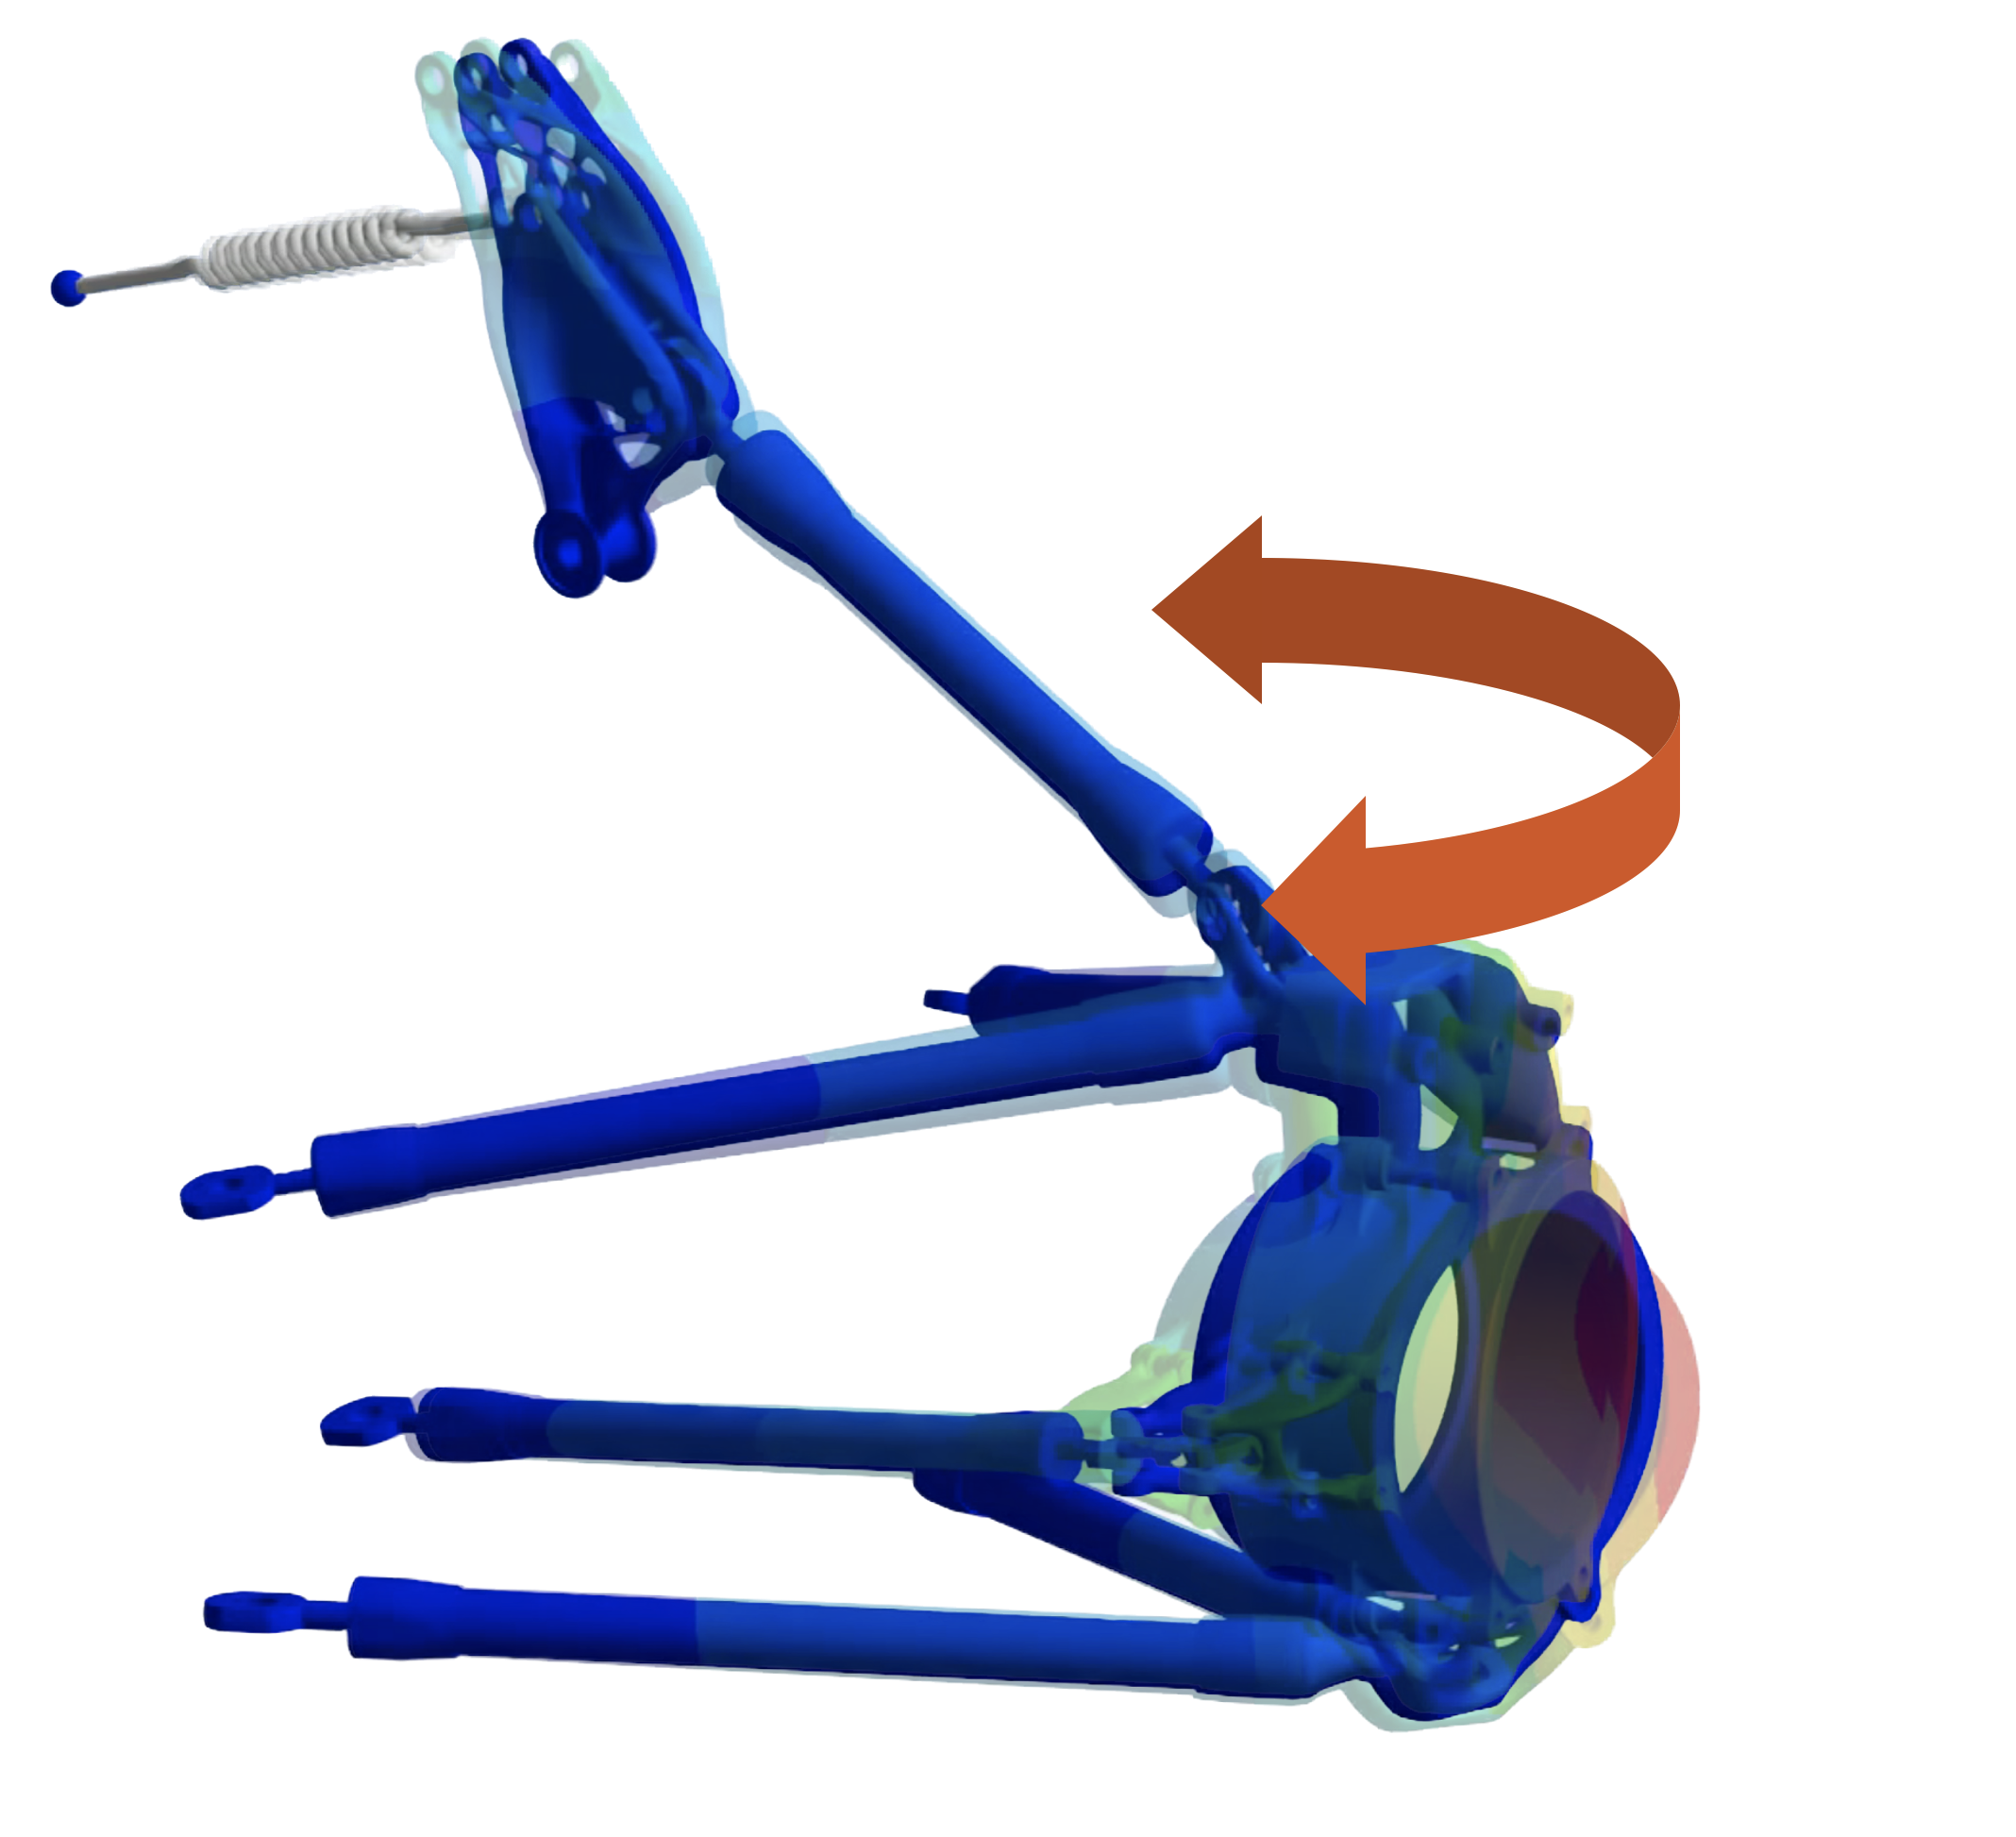
\includegraphics[width=0.5\linewidth]{mode2.png} \raisebox{2.0em}{\small{$f = 88.5$ Hz}} \\
    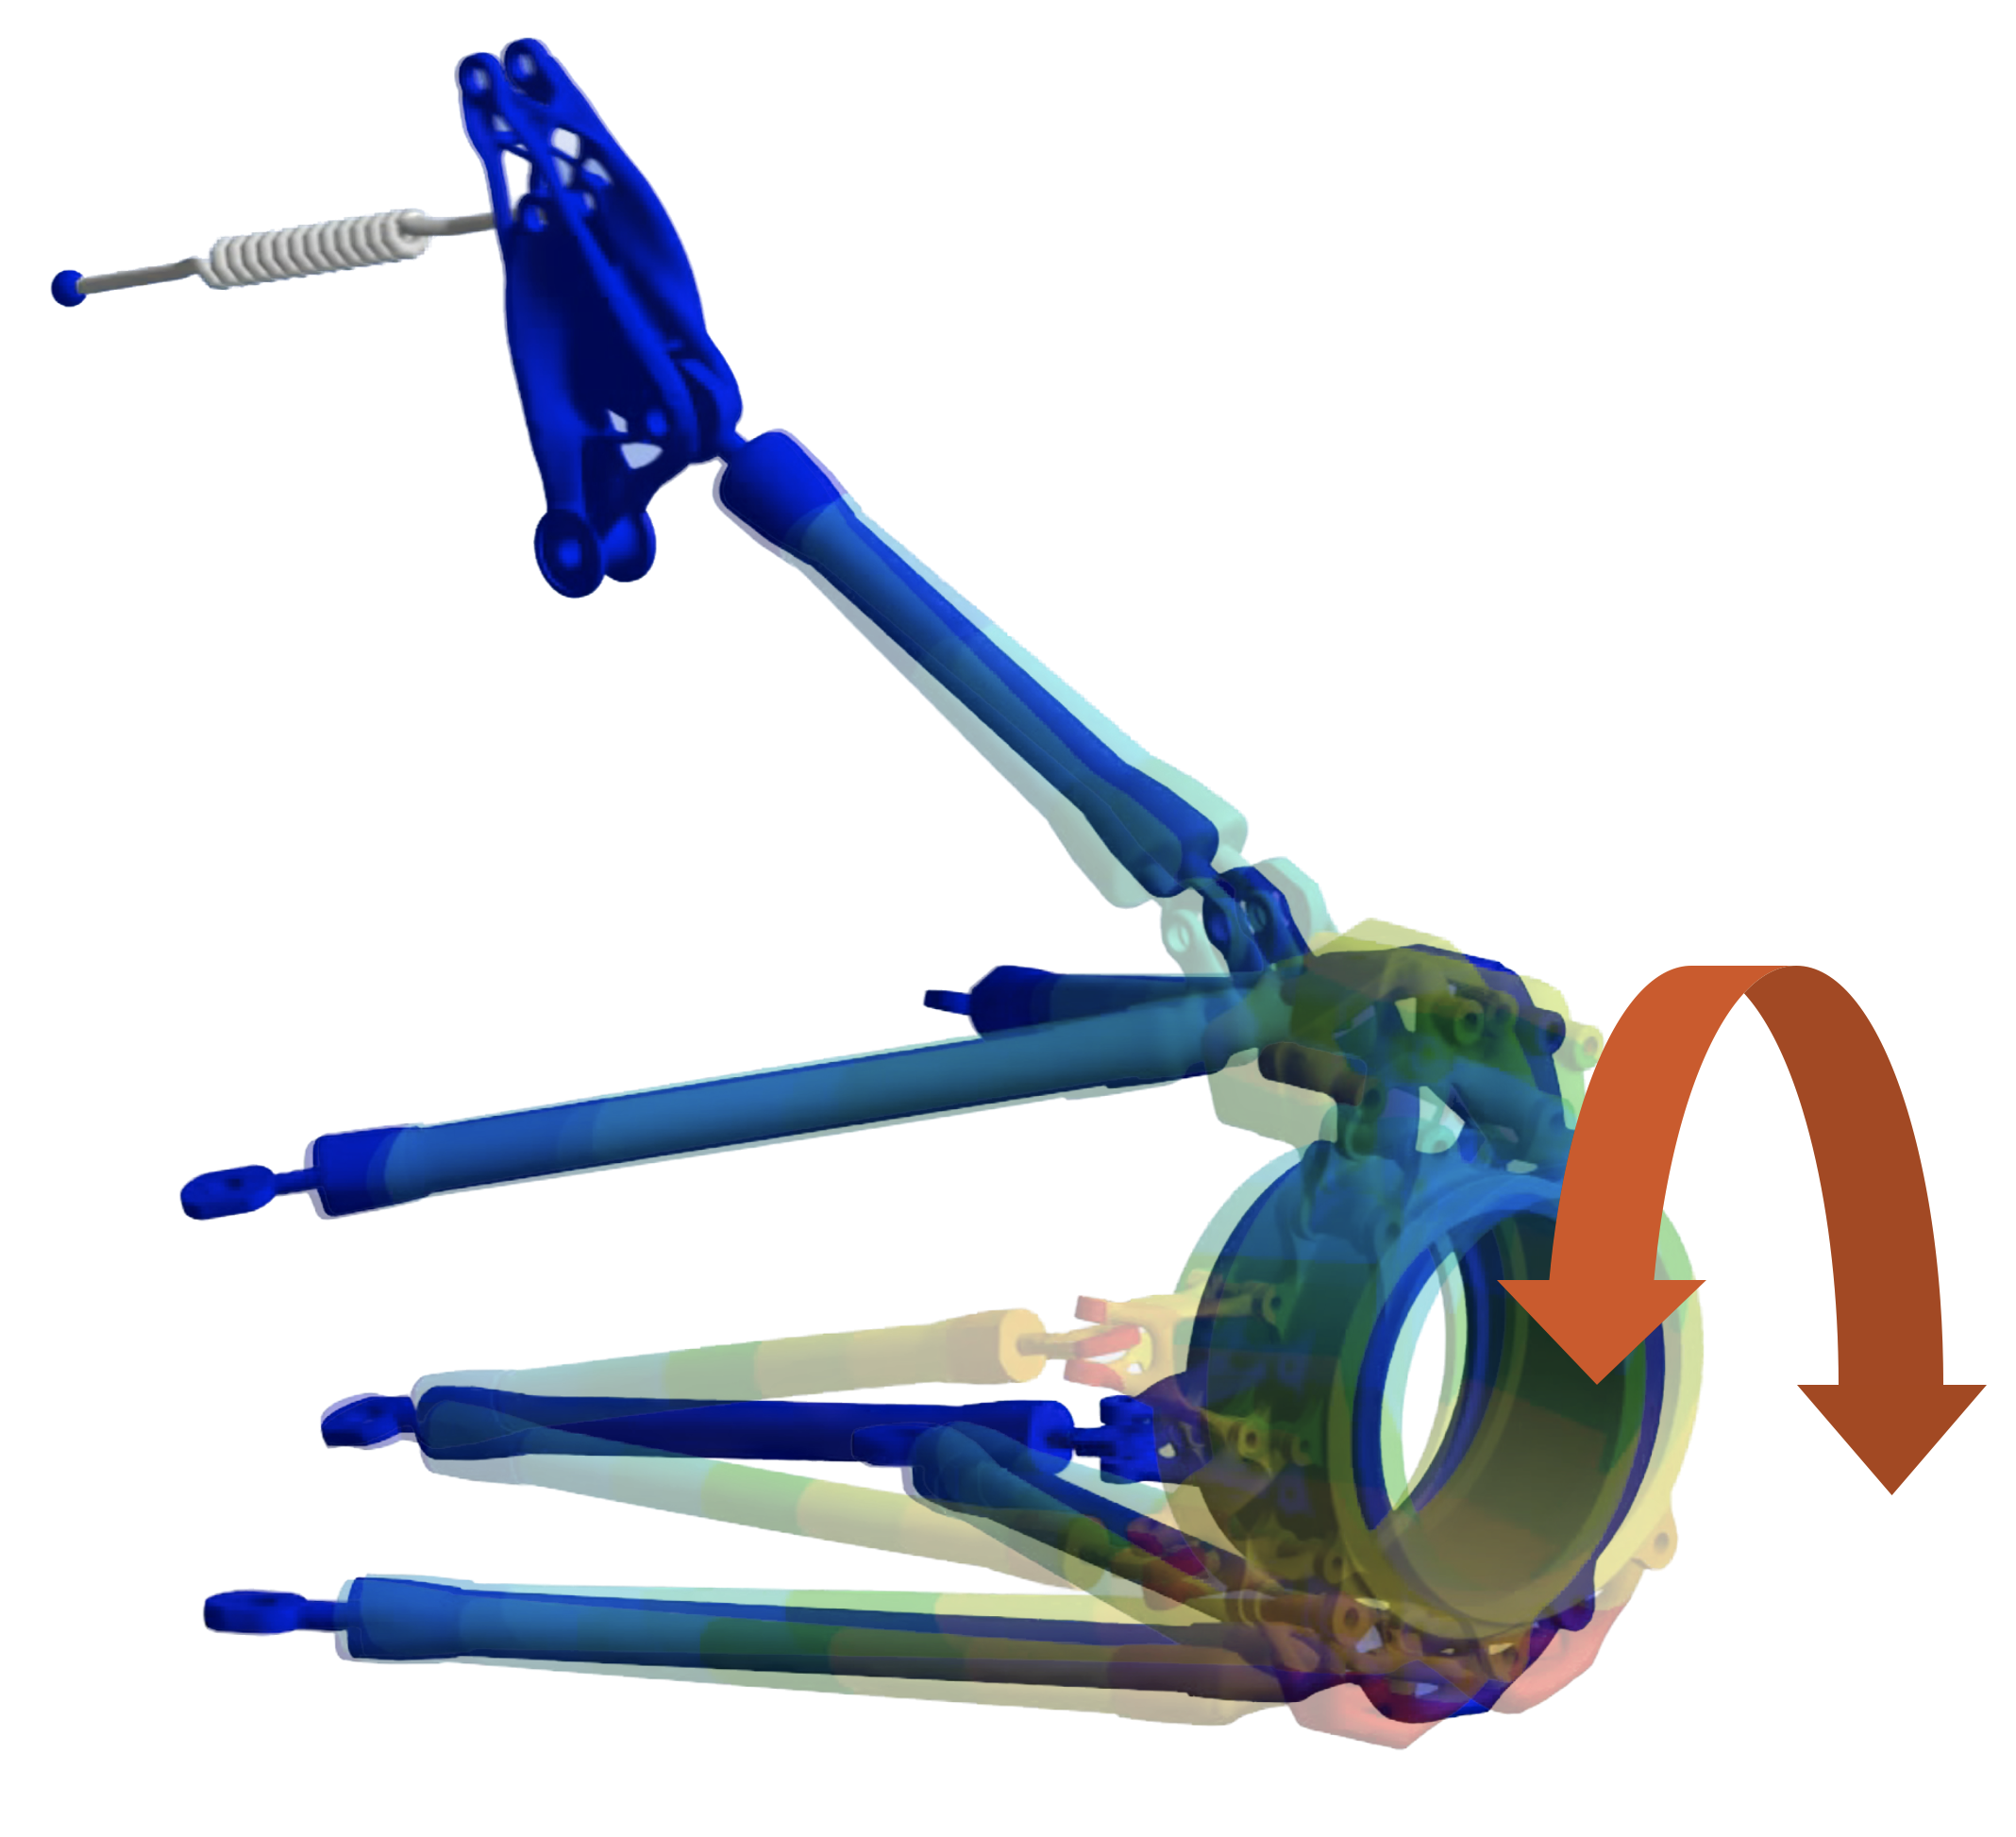
\includegraphics[width=0.5\linewidth]{mode3.png} \raisebox{2.0em}{\small{$f = 159.7$ Hz}} \\
  \end{minipage}
\end{frame}

\begin{frame}{Simulation results}{Full Vehicle Simulation}
  \begin{columns}
  \begin{column}{0.55\textwidth}
    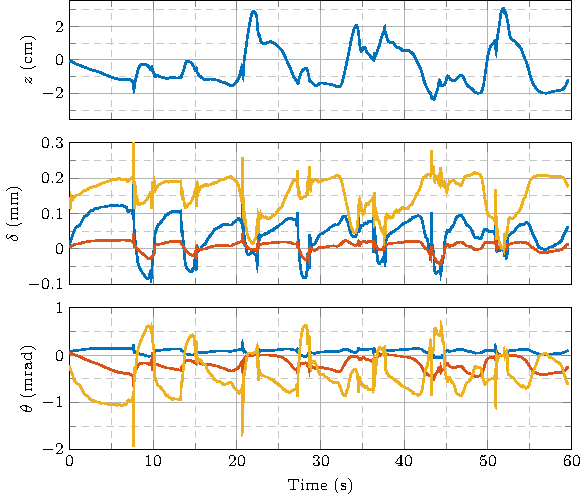
\includegraphics[width=0.95\textwidth]{compliance_PA.pdf}\\
    \emph{Legend}: {\color{mycolor1}$\blacksquare$} $x$-, {\color{mycolor2}$\blacksquare$} $y$-, {\color{mycolor3}$\blacksquare$} $z$-component.
  \end{column}
  \begin{column}{0.47\textwidth}
    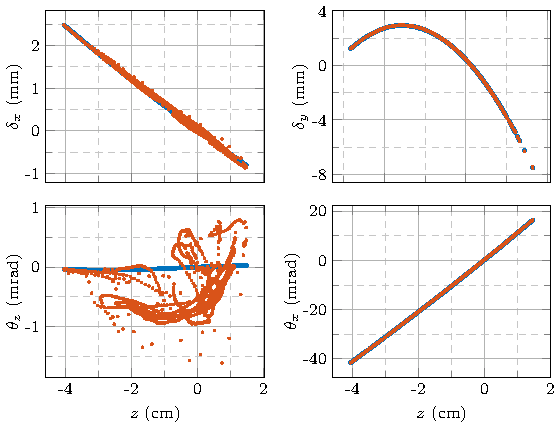
\includegraphics[width=1.0\textwidth]{kine_compliance_PA.pdf}\\
    \emph{Legend}: {\color{mycolor1}$\blacksquare$} kinematic, {\color{mycolor2}$\blacksquare$} total.
  \end{column}
  \end{columns}
\end{frame}

\begin{frame}{Simulation results}{Timing}
  \begin{center}
  \begin{table}[ht]
    \centering
    \begin{tabular}{p{0.3\textwidth}ccccc}
      \toprule
      \textbf{Compliance} & \multicolumn{4}{c}{\textbf{Computation time}} \\ \cmidrule(l{5pt}r{5pt}){2-5}
      \textbf{model} & $\mu$\,(\si{\micro\second}) & $\min$\,(\si{\micro\second}) & $\max$\,(\si{\micro\second}) & $\sigma^2$\,(\si{\micro\second\squared}) \\
      \midrule
      Compliance maps (linear) & $\phantom{0}40$ & $\phantom{0}4$ & $\phantom{0}48$ & $\phantom{0}1.2$ \\
      Compliance maps (cubic)  & $193$           & $84$           & $880$           & $42.9$ \\
      Symbolic FEM             & $181$           & $42$           & $417$           & $45.2$ \\
      \bottomrule
    \end{tabular}
  \end{table}
\end{center}
\end{frame}

\section{Tire-Road Interaction Modelling}

\begin{frame}{Geometry Library}
  \vspace{-1.0em}%
  \centering%
  \begin{minipage}[c]{0.45\textwidth}%
    \centering\def\svgwidth{6.5cm}%
    \small{\input{figures/acme_entities_1.pdf_tex}} \\
    \def\svgwidth{6.5cm}%
    \small{\input{figures/acme_entities_2.pdf_tex}}
  \end{minipage}%
  \hfill%
  \begin{minipage}[c]{0.45\textwidth}%
    \centering\def\svgwidth{6.5cm}%
    \small{\input{figures/acme_collection.pdf_tex}}
  \end{minipage}%
\end{frame}

\begin{frame}{Tire-Road Interaction Model}
  \vspace{-1.0em}
  \centering
  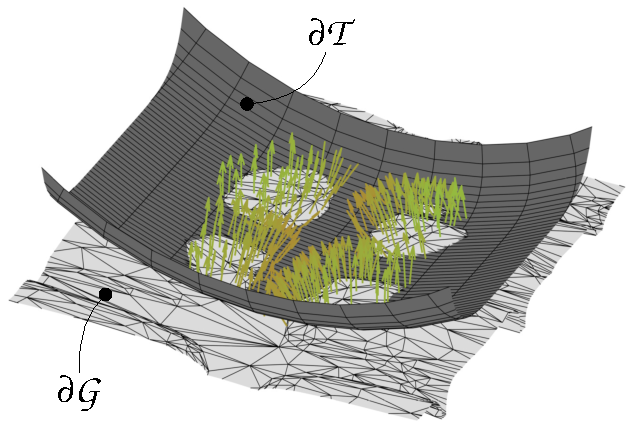
\includegraphics[width=0.3\textwidth]{zoom_ipe.pdf}%
  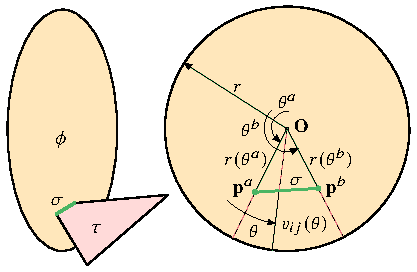
\includegraphics[width=0.35\textwidth]{intersection.pdf} \\
  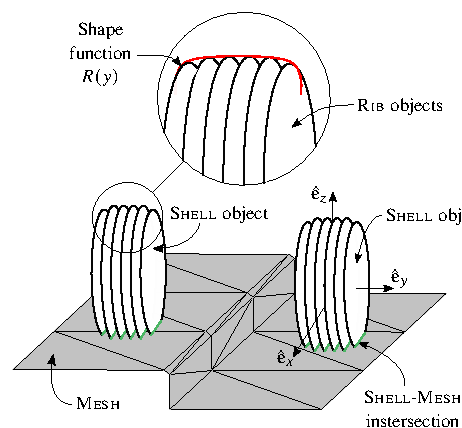
\includegraphics[width=0.3\textwidth]{tire_zoom.pdf}%
  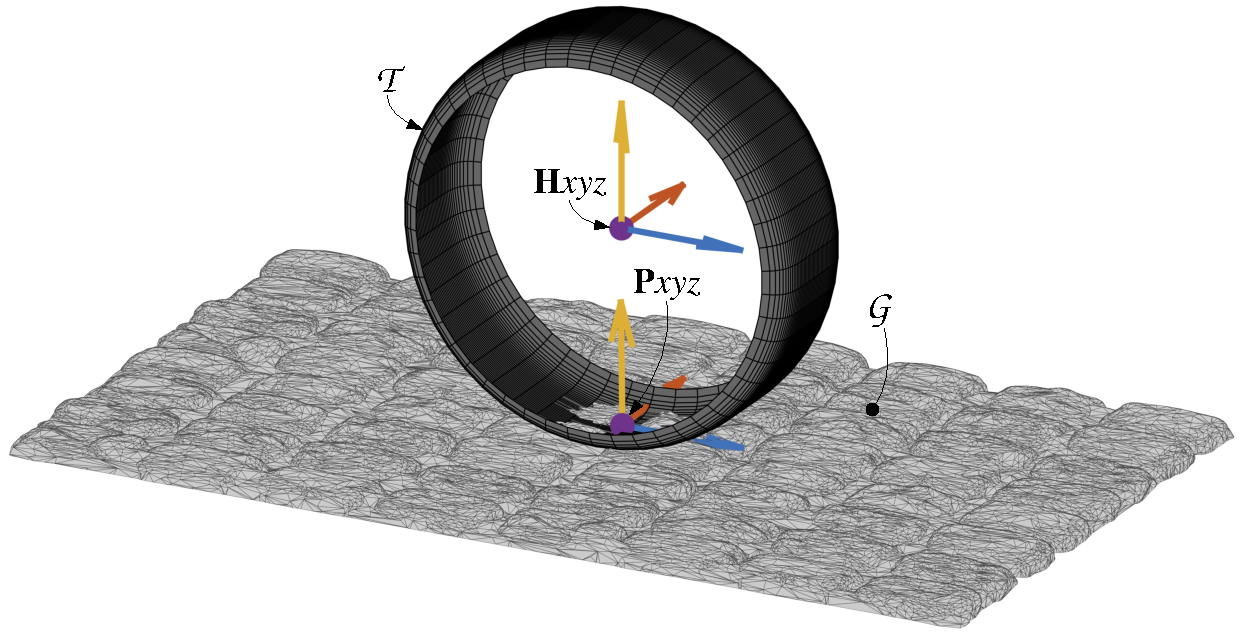
\includegraphics[width=0.5\textwidth]{road_shell_ipe.pdf}
\end{frame}

\begin{frame}{Tire-Road Interaction Model}
  \vspace{-1.0em}
  \centering
  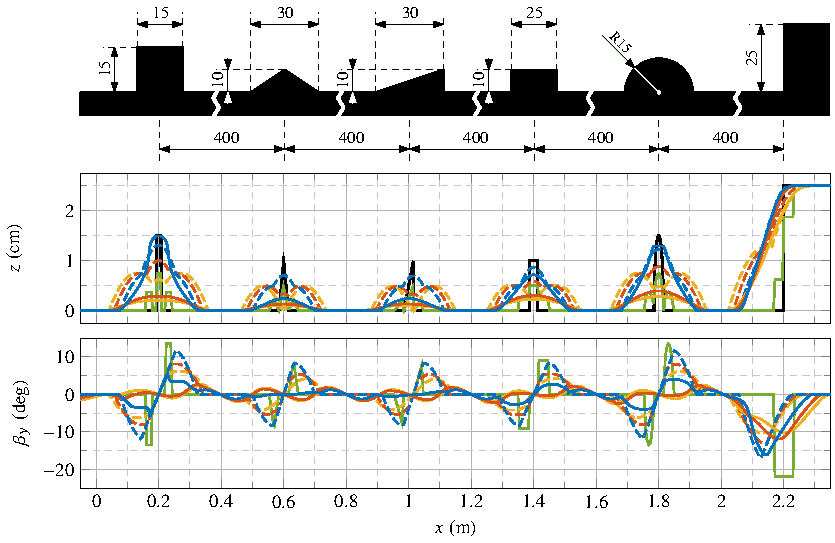
\includegraphics[width=0.6\textwidth]{steps.pdf}%
  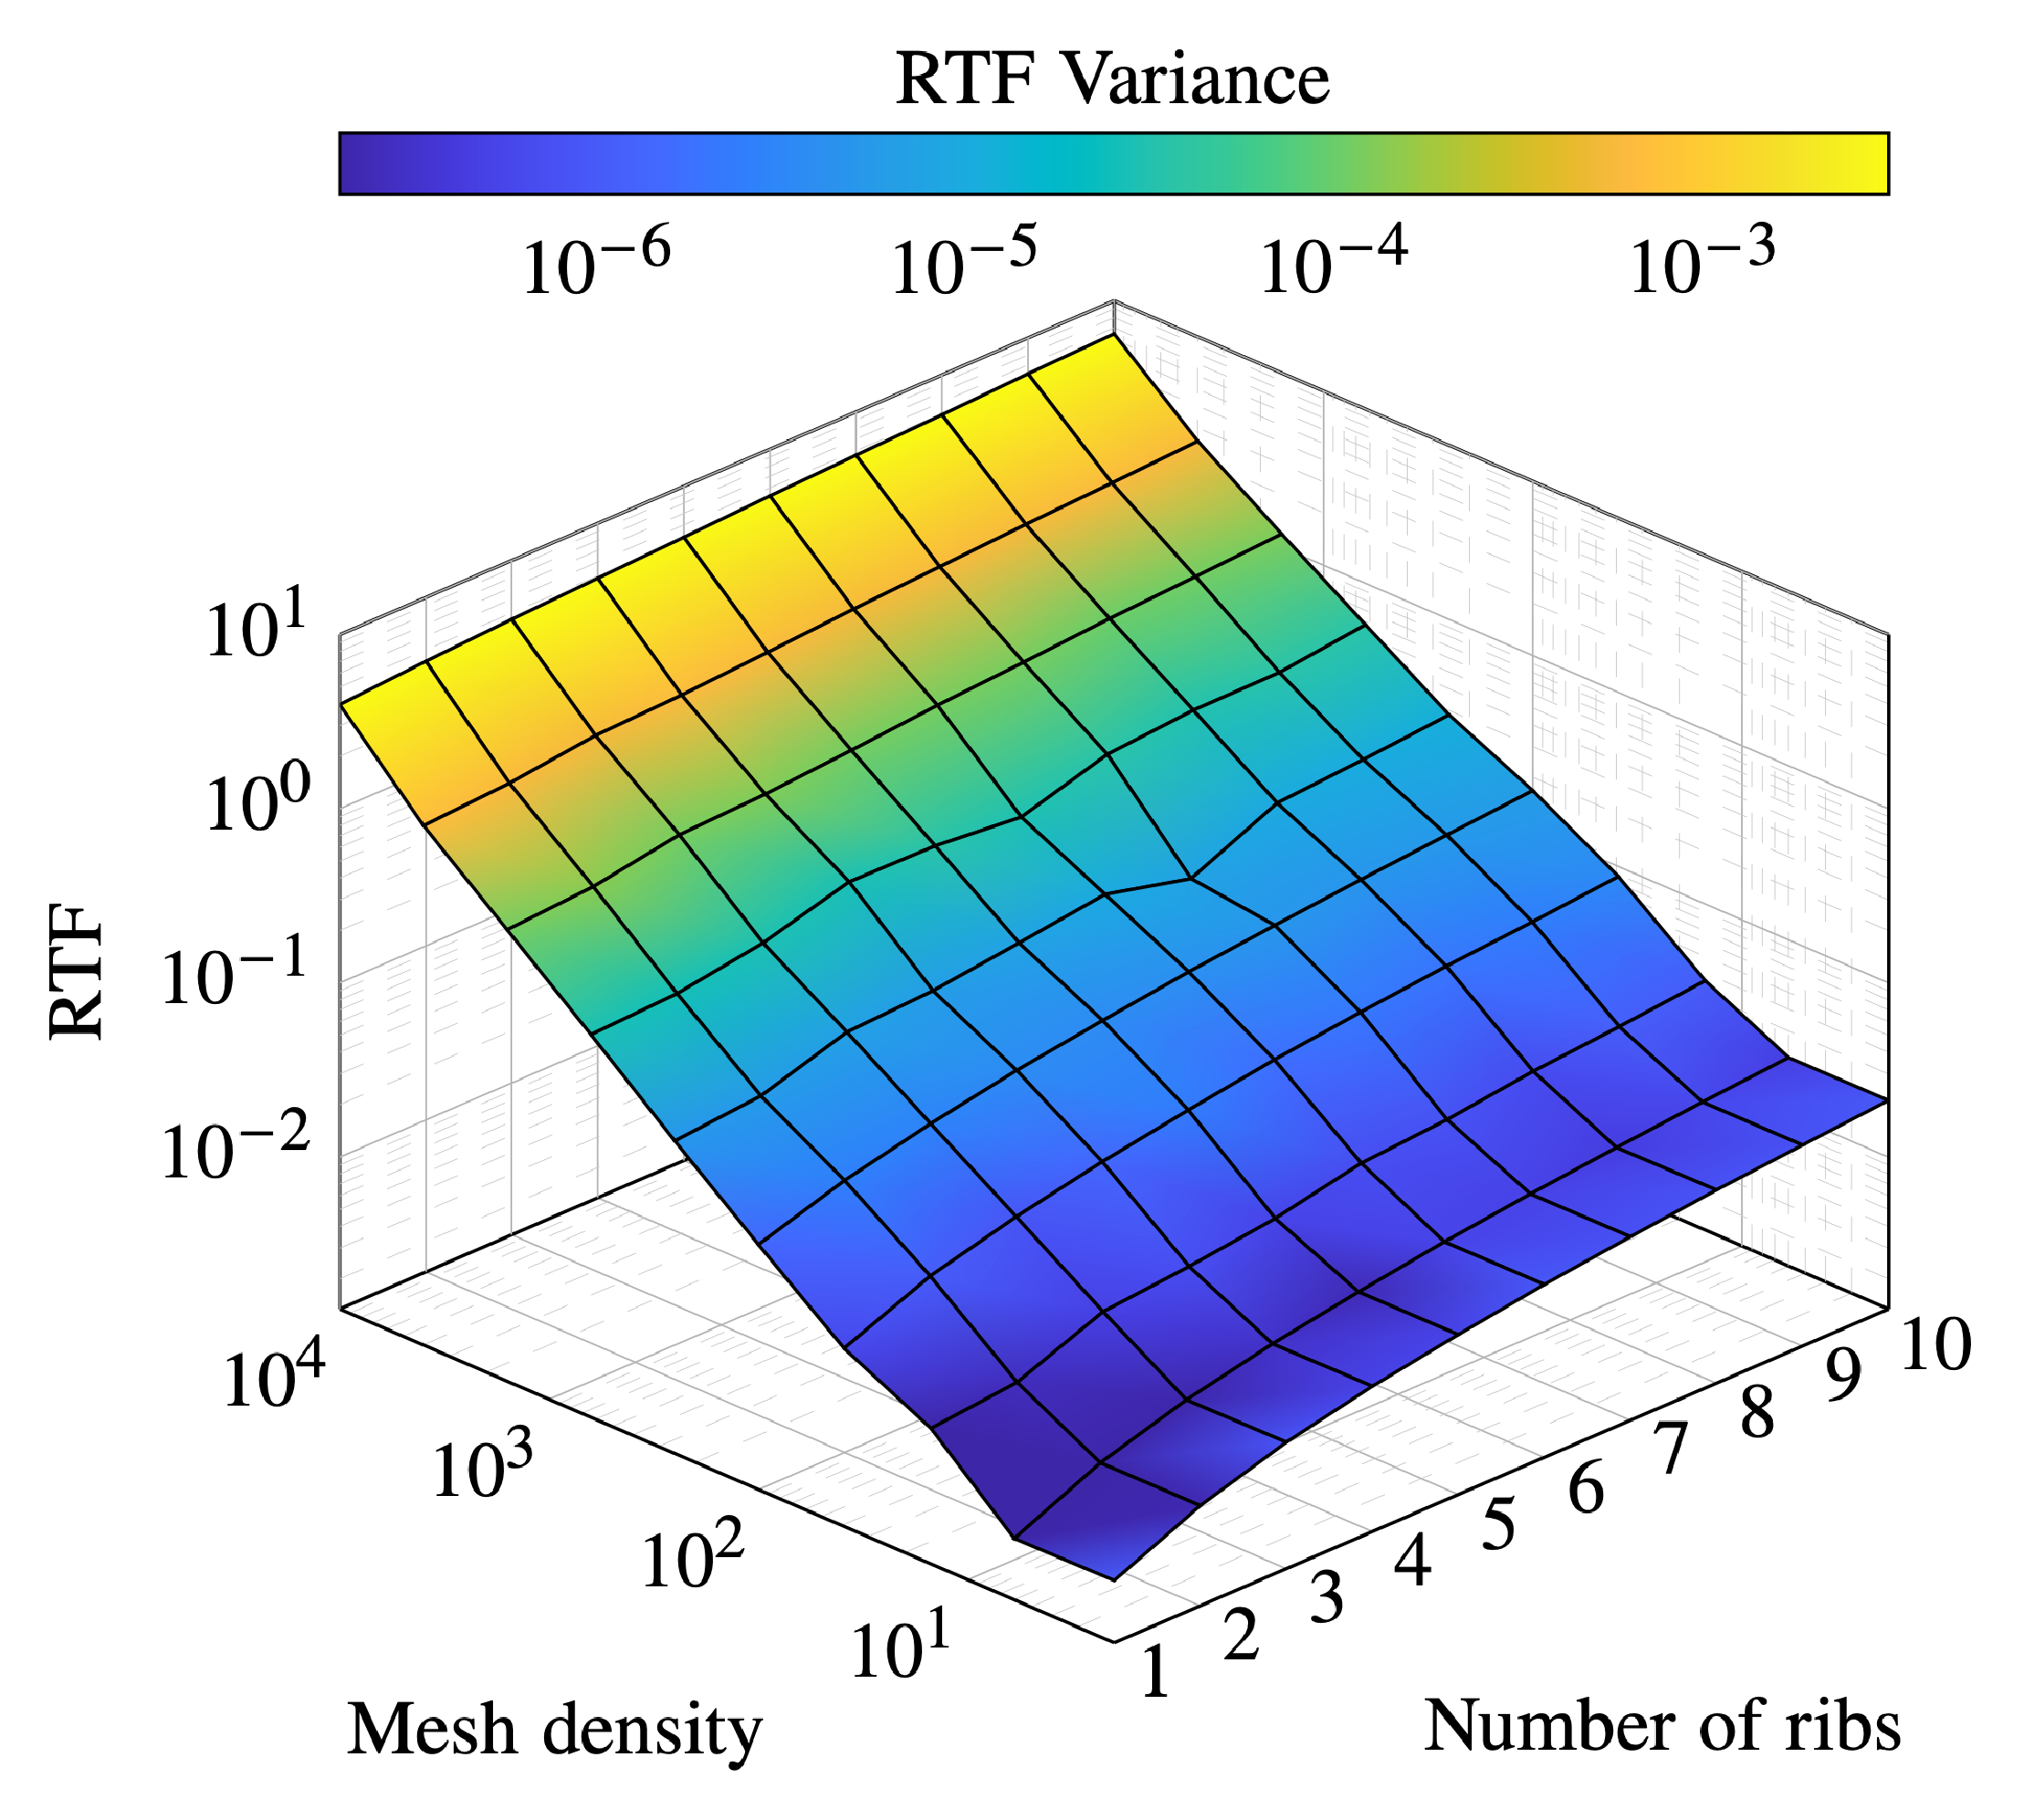
\includegraphics[width=0.4\textwidth]{rtf_enve.pdf}
\end{frame}

\begin{frame}{Brush Tire Model}
  \vspace{-1.0em}
  \centering
  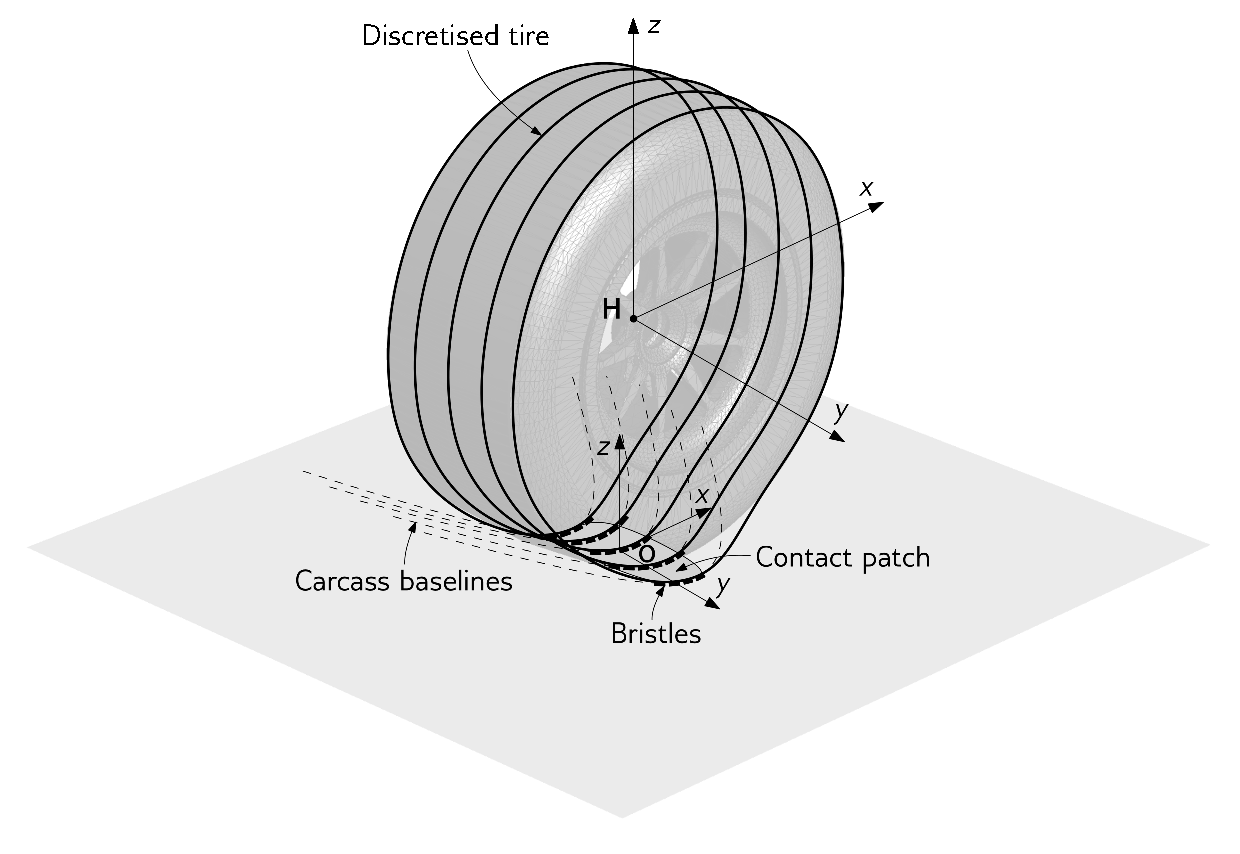
\includegraphics[width=0.75\textwidth]{brush_model.eps}
\end{frame}

\begin{frame}{Brush Tire Model}
  \vspace{-1.0em}
  \centering
  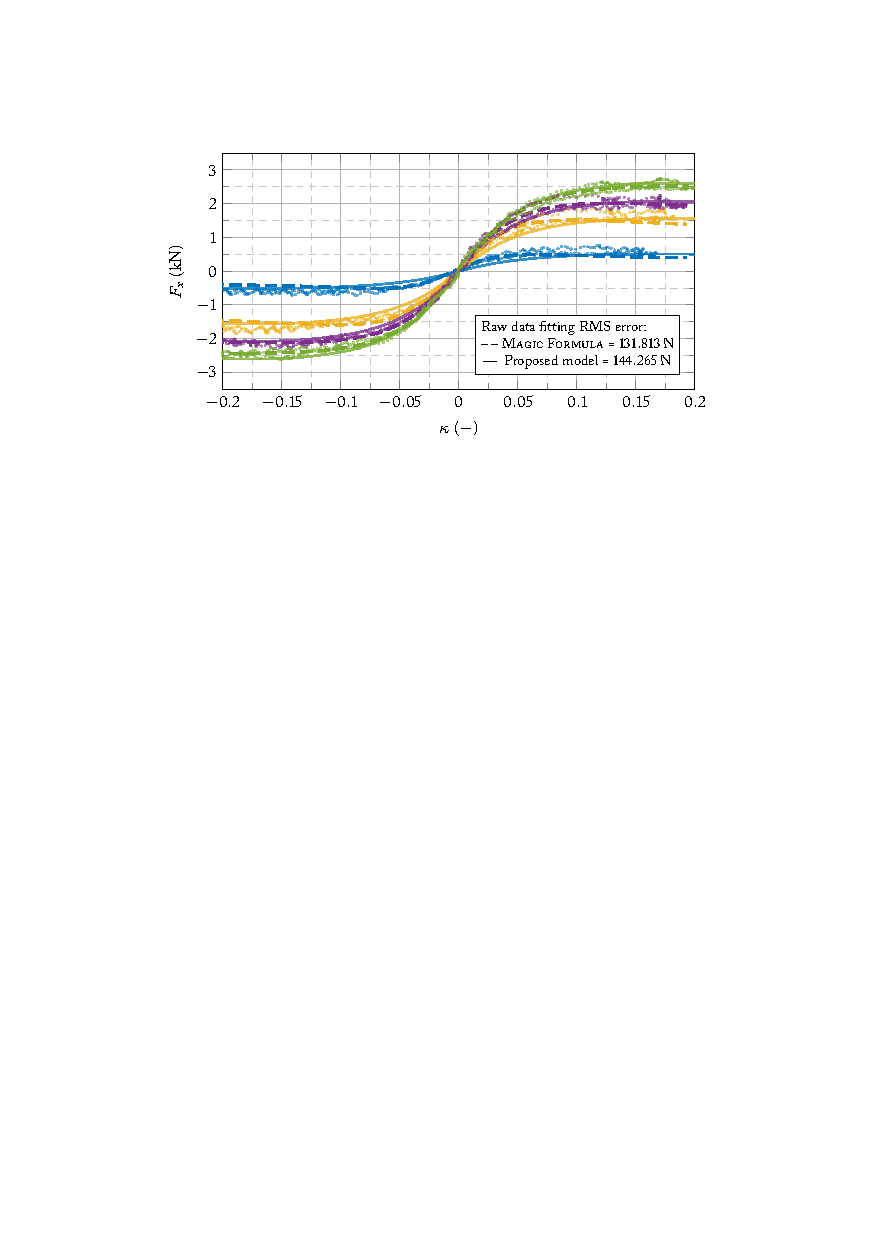
\includegraphics[width=0.475\textwidth]{fx_tire.pdf}%
  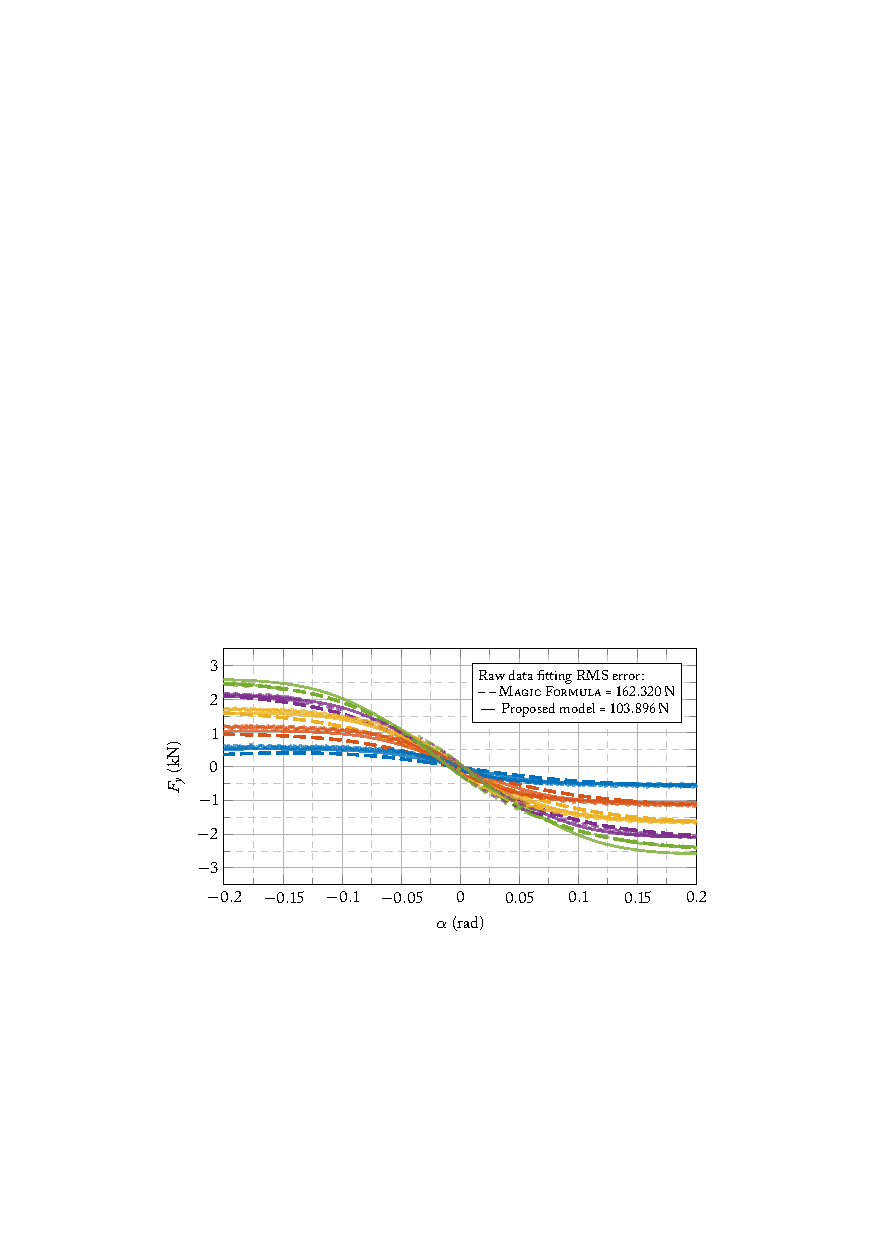
\includegraphics[width=0.475\textwidth]{fy_tire.pdf} \\
  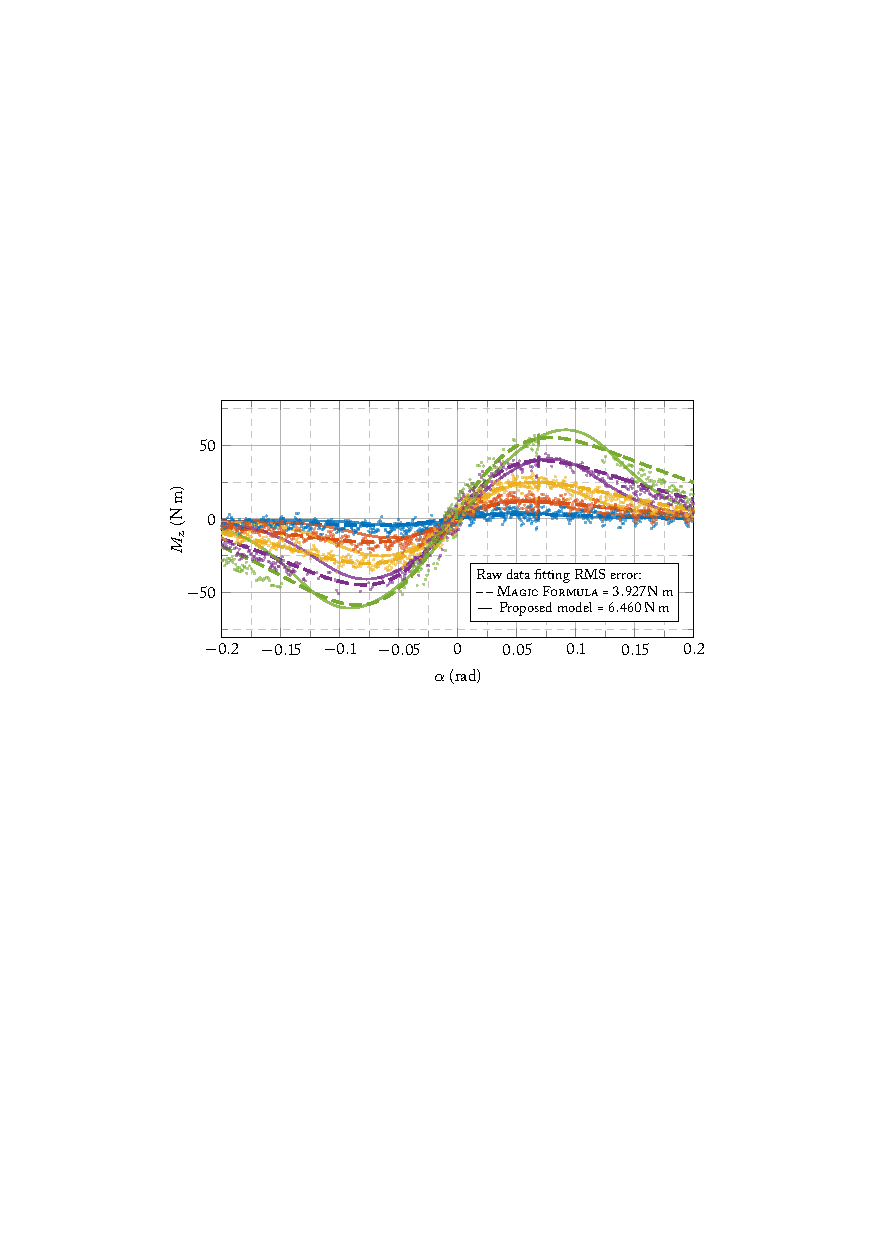
\includegraphics[width=0.475\textwidth]{mz_tire.pdf}
\end{frame}

\begin{frame}{Brush Tire Model}
  \vspace{-1.0em}
  \centering
  \small{\begin{tabularx}{0.8\textwidth}{*{6}{Y}}%{\textwidth}{*{14}{Y}}
    %\multicolumn{14}{c}{\textbf{Quasi-Newton Methods Performance with 5 Ribs}} \\
    \multicolumn{6}{c}{\textbf{Quasi-Newton Methods Performance with 5 Ribs}} \\
    \toprule
    \multirow{2.25}{*}{\textbf{Method}} &
    %\multicolumn{4}{c}{\textbf{Evaluations} ($-$)} &
    %\multicolumn{4}{c}{\textbf{Iterations} ($-$)} &
    \multicolumn{4}{c}{\textbf{Time} (\USI{\micro\second})} &
    \multirow{2}{*}{\textbf{Success}} \\
    \cmidrule(l{4pt}r{4pt}){2-5}
    %\cmidrule(l{4pt}r{4pt}){6-9}
    %\cmidrule(l{4pt}r{4pt}){10-13}
    %& \mini{} & \maxi{} & \meai{} & \vari{} & \mini{} & \maxi{} & \meai{} & \vari{}
      & \mini{} & \maxi{} & \meai{} & \vari{} & \\
    \midrule
    PIM   %& $100$ & $100$ & $100.0$ & $0.00$    & $100$ & $100$ & $100.0$ & $0.0$
      & $518.0$ & $7949.0$ & $617.2$  & $13953.2$  & $0.0\%$   \\ %\hline
    G1M   %& $-$   & $-$   & $-$     & $-$       & $-$   & $-$   & $-$     & $-$
      & $-$     & $-$      & $-$      & $-$        & Overflow  \\ %\hline
    G2M   %& $4$   & $100$ & $9.2$   & $55.8$    & $4$   & $100$ & $9.2$   & $55.8$
      & $23.5$  & $1089.4$ & $69.0$   & $5252.0$   & $99.5\%$  \\ %\hline
    ENM   %& $6$   & $200$ & $11.9$  & $234.0$   & $3$   & $100$ & $6.5$   & $58.5$
      & $25.0$  & $2025.0$ & $81.5$   & $11002.8$  & $99.4\%$  \\ %\hline
    BBM   %& $-$   & $-$   & $-$     & $-$       & $-$   & $-$   & $-$     & $-$
      & $-$     & $-$      & $-$      & $-$        & $0.0\%$   \\ %\hline
    BGM   %& $4$   & $100$ & $8.8$   & $18.4$    & $4$   & $100$ & $8.8$   & $18.4$
      & $22.6$  & $948.1$  & $62.5$   & $1973.0$   & $99.9\%$  \\ %\hline
    BCM   %& $4$   & $17$  & $8.4$   & $6.7$     & $4$   & $17$  & $8.4$   & $6.7$
      & $22.9$  & $264.4$  & $55.7$   & $885.9$    & $100.0\%$ \\ %\hline
    D-PIM %& $100$ & $496$ & $190.7$ & $13628.1$ & $100$ & $100$ & $100.0$ & $0.0$
      & $507.0$ & $5383.0$ & $1151.9$ & $568491$   & $0.0\%$   \\ %\hline
    D-G1M %& $-$   & $-$   & $-$     & $-$       & $-$   & $-$   & $-$     & $-$
      & $-$     & $-$      & $-$      & $-$        & Overflow  \\ %\hline
    D-G2M %& $4$   & $376$ & $11.3$  & $572.4$   & $4$   & $100$ & $9.3$   & $57.1$
      & $21.5$  & $3195.5$ & $80.4$   & $40321.9$  & $99.5\%$  \\ %\hline
    D-ENM %& $6$   & $513$ & $12.8$  & $829.7$   & $3$   & $100$ & $6.3$   & $44.3$
      & $27.0$  & $5207.7$ & $97.5$   & $52752.6$  & $99.5\%$  \\ %\hline
    D-BBM %& $4$   & $125$ & $11.0$  & $58.0$    & $4$   & $42$  & $9.3$   & $12.8$
      & $22.3$  & $1284.0$ & $76.9$   & $5126.3$   & $100.0\%$ \\ %\hline
    D-BGM %& $4$   & $376$ & $9.7$   & $110.6$   & $4$   & $100$ & $8.7$   & $15.1$
      & $21.3$  & $3238.9$ & $67.0$   & $8142.9$   & $99.9\%$  \\ %\hline
    D-BCM %& $4$   & $35$  & $9.1$   & $14.6$    & $4$   & $17$  & $8.4$   & $6.7$
      & $22.5$  & $316.8$  & $62.1$   & $1615.1$   & $100.0\%$ \\
    \bottomrule
  \end{tabularx}}%
\end{frame}

\begin{frame}{Brush Tire Model}
    \vspace{-1.0em}
    \centering
    \small{\begin{tabularx}{0.75\textwidth}{*{6}{Y}}%{\textwidth}{*{14}{Y}}
    %\multicolumn{14}{c}{\textbf{Broyden Combined Method Performance}} \\
    \multicolumn{6}{c}{\textbf{Broyden Combined Method Performance}} \\
    \toprule
    \multirow{2.25}{*}{\textbf{Ribs}} &
    %\multicolumn{4}{c}{\textbf{Evaluations} ($-$)} &
    %\multicolumn{4}{c}{\textbf{Iterations} ($-$)} &
    \multicolumn{4}{c}{\textbf{Time} (\USI{\micro\second})} &
    \multirow{2}{*}{\textbf{Success}} \\
    \cmidrule(l{4pt}r{4pt}){2-5}
    %\cmidrule(l{4pt}r{4pt}){6-9}
    %\cmidrule(l{4pt}r{4pt}){10-13}
    %\multirow{0.5}{*}{\textbf{of Ribs}}
    %& \mini{} & \maxi{} & \meai{} & \vari{} & \mini{} & \maxi{} & \meai{} & \vari{}
      & \mini{} & \maxi{} & \meai{} & \vari{} & \\
    \midrule
    $1$  %& $6$     & $11$    & $7.9$   & $10.3$
         %& $6$     & $11$    & $7.9$   & $10.3$
         & $12.1$  & $89.0$  & $19.4$  & $20.6$  & $100.0\%$ \\ %\hline
    $5$  %& $4$     & $17$    & $7.9$   & $10.3$
         %& $4$     & $17$    & $7.9$   & $10.3$
         & $22.9$  & $264.4$ & $55.7$  & $885.9$ & $100.0\%$ \\ %\hline
    $10$ %& $6$     & $11$    & $7.9$   & $10.3$
         %& $6$     & $11$    & $7.9$   & $10.3$
         & $106.9$ & $361.8$ & $167.3$ & $1746.22$ & $100.0\%$ \\ %\hline
    $15$ %& $6$     & $11$    & $7.9$   & $10.3$
         %& $6$     & $11$    & $7.9$   & $10.3$
         & $158.0$ & $523.5$ & $249.4$ & $3878.2$ & $100.0\%$ \\ %\hline
    $20$ %& $6$     & $11$    & $7.9$   & $10.3$
         %& $6$     & $11$    & $7.9$   & $10.3$
         & $210.1$ & $693.3$ & $332.9$ & $7028.7$ & $100.0\%$ \\ %\hline
    $25$ %& $6$     & $11$    & $7.9$   & $10.3$
         %& $6$     & $11$    & $7.9$   & $10.3$
         & $262.7$ & $858.4$ & $414.0$ & $10708.3$ & $100.0\%$ \\
    \bottomrule
  \end{tabularx}}%
\end{frame}

% That's all Folks!